\documentclass{beamer}
\usepackage{pgfpages}
\usepackage{algorithm2e}
\usepackage{complexity}

\usetheme{Pittsburgh}
\useinnertheme{rectangles}
\usefonttheme{serif}
\newcommand{\T}{\mathcal{T}}

\newcommand{\tup}[1]
           {
             \relax\ifmmode
             \langle #1 \rangle
             \else $\langle$ #1 $\rangle$ \fi
           }

\title{\textbf{Automatic Dynamic Parallelotope Bundles for Reachability of Nonlinear Dynamical Systems}}

\author{\textbf{Edward Kim}\inst{1}}
\institute{\inst{1}University of North Carolina at Chapel Hill}

\begin{document}

\begin{frame}
\titlepage
\end{frame}

%\begin{frame}
%\frametitle{Introduction}
%\begin{enumerate}
%\end{enumerate}
%\end{frame}


%\begin{frame}
%\frametitle{Outline}
%\begin{enumerate}
%  \item Overview of Background
%  \item Our Contributions
%  \item Presentation of Algorithm
%  \item Results on Benchmarks
%  \item Concluding Remarks
%\end{enumerate}
%\end{frame}

\begin{frame}
  \frametitle{\textbf{Background:} Reachability Computation}
  \begin{columns}
      \column{0.5\textwidth}\footnotesize
        \begin{enumerate}
          \item Reachable set computation is an instrumental tool in performing safety analysis over dynamical systems.
          \item These computations involve taking an initial set of states and propagating them for a set amount of time to understand the possible states the initial states could reach within the alloted time.
          \item Techniques for good over-approximation of reachable sets over classes of \emph{non-linear} systems are topics of active research.
        \end{enumerate}
        \hspace{3em}
        \column{0.6\textwidth}
        \begin{figure}
            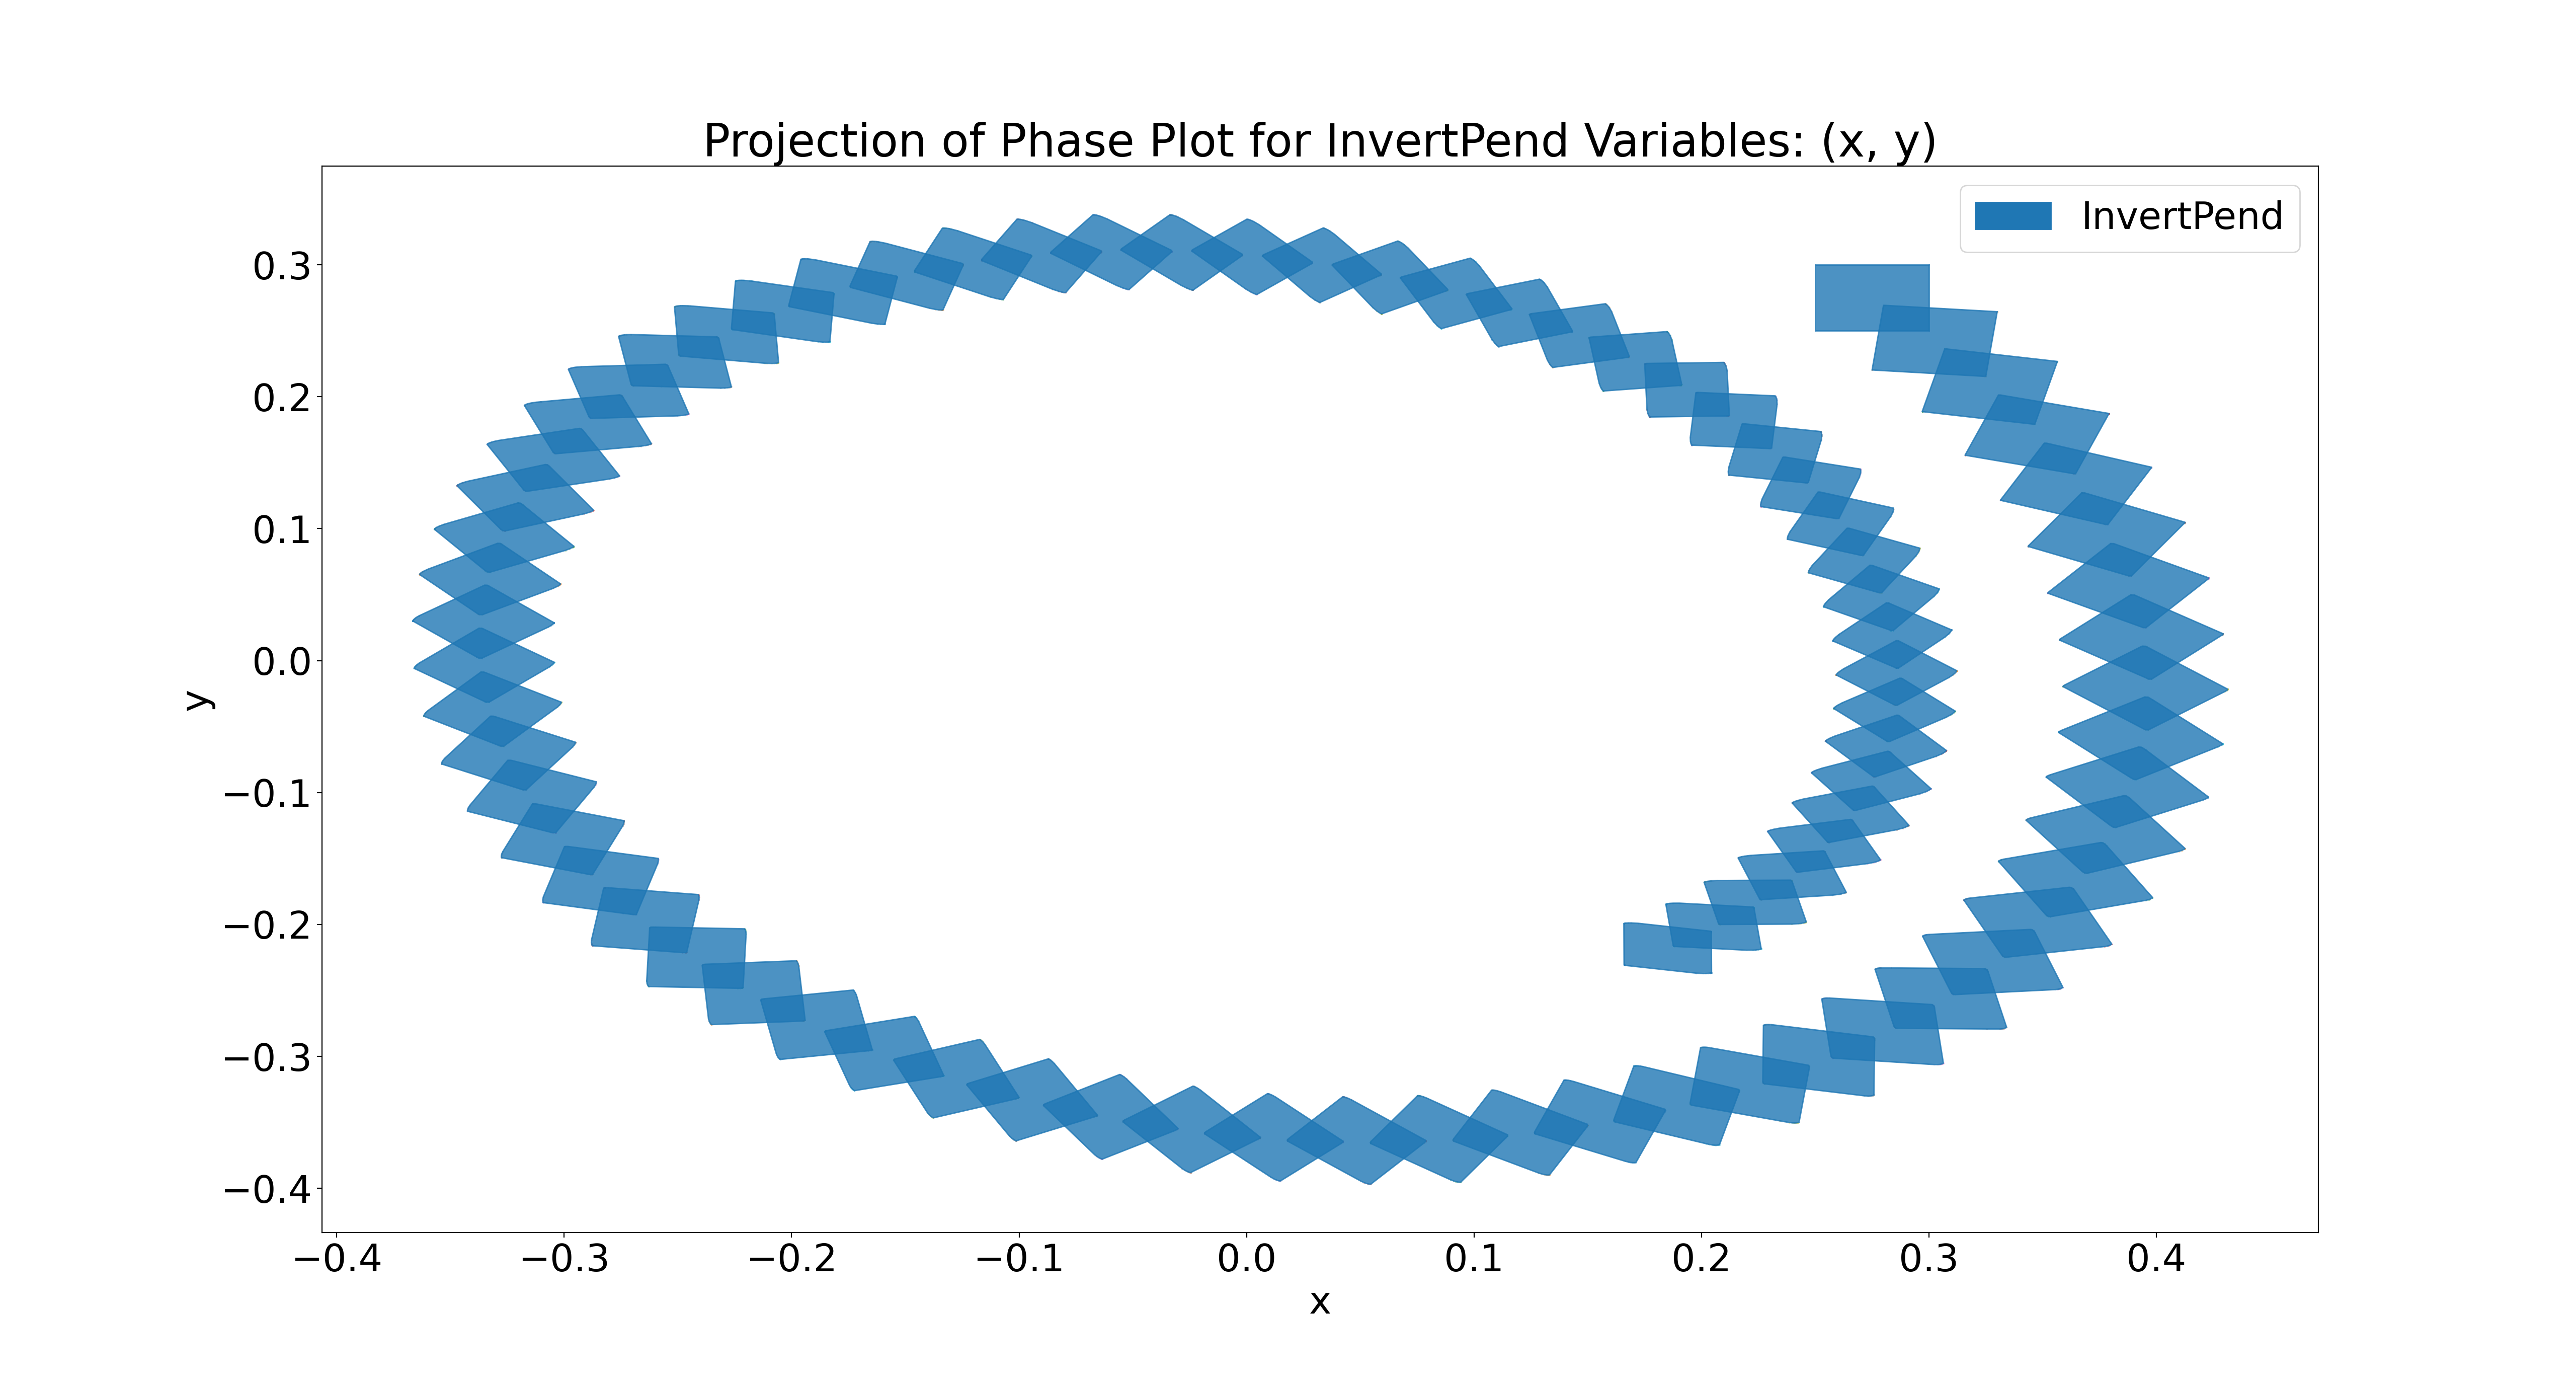
\includegraphics[width=1.13\textwidth]{InvertPend}
            \caption{Plot of Inverted Pendulum System under Initial Conditions $x \in [0.25, 0.3], y \in [0.25, 0.3]$}
          \end{figure}
\end{columns}
\end{frame}

\begin{frame}
  \frametitle{\textbf{Background:} Reachability Computation}
  \begin{enumerate}
    \item The state of a system, denoted as $x$, lies in a domain $D \subseteq \mathbb{R}^n$.
    A discrete-time nonlinear system is denoted as
    \begin{equation}
      x^{+} = f(x)
    \end{equation}
    where $f: \mathbb{R}^{n} \rightarrow \mathbb{R}^{n}$ is a nonlinear function.
    \item The trajectory of a system that evolves according to $f$, denoted as $\xi(x_0)$ is a sequence $x_0, x_1, \ldots $ where $x_{i+1} = f(x_i)$.
    \item The $k^{th}$ element in this sequence $x_k$ is denoted as $\xi(x_0,k)$.
  \end{enumerate}
\end{frame}

\begin{frame}
  \frametitle{\textbf{Background:} Reachability Computation}
  \begin{enumerate}
  \item Given an initial set $\Theta \subseteq \mathbb{R}^n$, the \emph{reachable set} at step $k$, denoted as $\Theta_k$ is defined as
  \begin{equation*}
    \Theta_k = \{ \xi(x,k)\: | \: x \in \Theta\}
  \end{equation*}
  \item Setting number of steps $n$ and $\Theta_0 = \Theta$, the total reachable set for $n$ steps can be defined as
  \begin{equation*}
    \mathcal{R} = \bigcup_{k=0}^n \{ \xi(x,k)\: | \: x \in \Theta\}
  \end{equation*}
  \end{enumerate}
\end{frame}

\begin{frame}
  \frametitle{\textbf{Background:} Reachability with Template Polyhedra}
  \begin{enumerate}
  \item One of many techniques in computing the overapproximation of the reachable sets for discrete non-linear systems is to use \textbf{template polyhedra} to bound the reachable set.
  \item Study of template polyhedra find motivations in the static analysis of programs
  \item We are particularly interested in \emph{parallelotopes} as our template polyhedra.
\end{enumerate}
\end{frame}

\begin{frame}
  \frametitle{\textbf{Background:} Reachability with Template Polyhedra}
  \begin{definition}
    For $\mathbb{R}^n$, a \emph{template polyhedron} is expressed a tuple $\langle H, \textbf{d} \rangle$ where $H$ is an $m \times n$ real-valued matrix and $\textbf{d} \in \mathbb{R}^n$ is a real-valued vector. The polyhedron is defined by the conjunction of linear inequalities
    \[ \bigwedge_{i=1}^m H_i\cdot \textbf{x} \leq d_i \]
    where $H_i$ is the $i^{th}$ row of template matrix $H$ and $\textbf{x} = (x_1, \cdots, x_m)$
  \end{definition}
\end{frame}

\begin{frame}
  \frametitle{\textbf{Background:} Parallelotope Intuition}
  \begin{figure}
    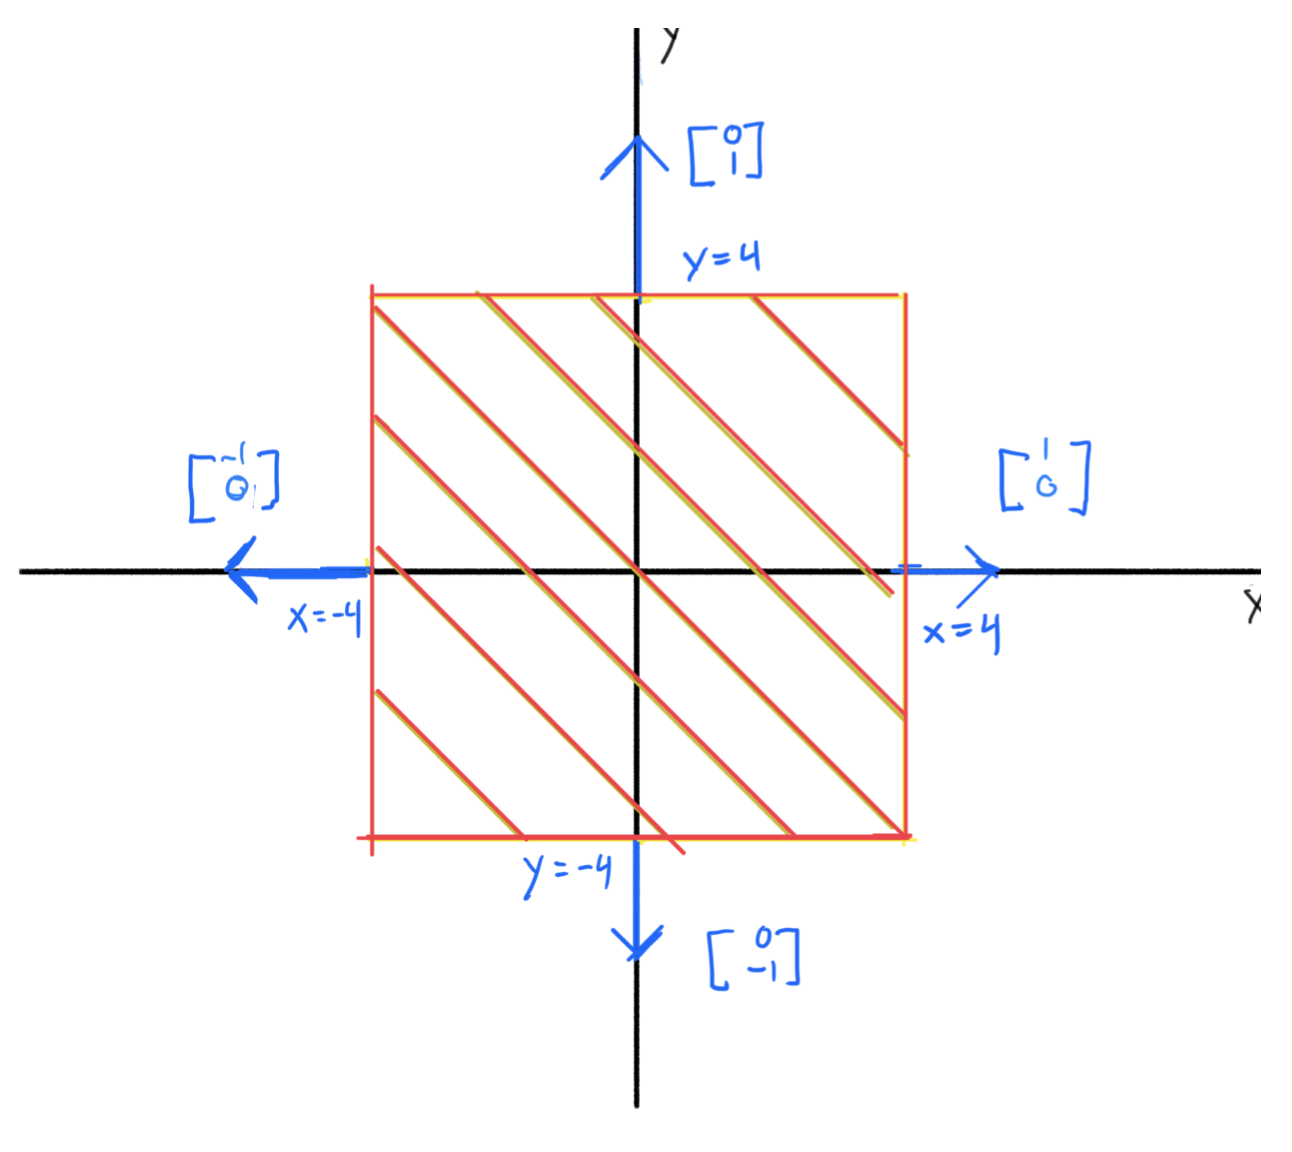
\includegraphics[width=0.7\textwidth]{ptopeiniti}
    \caption{Example Initial Parallelotope with offset distance of 4 for all template directions}
  \end{figure}
\end{frame}

\begin{frame}
  \frametitle{\textbf{Background:} Parallelotope Matrices}
  \begin{figure}
    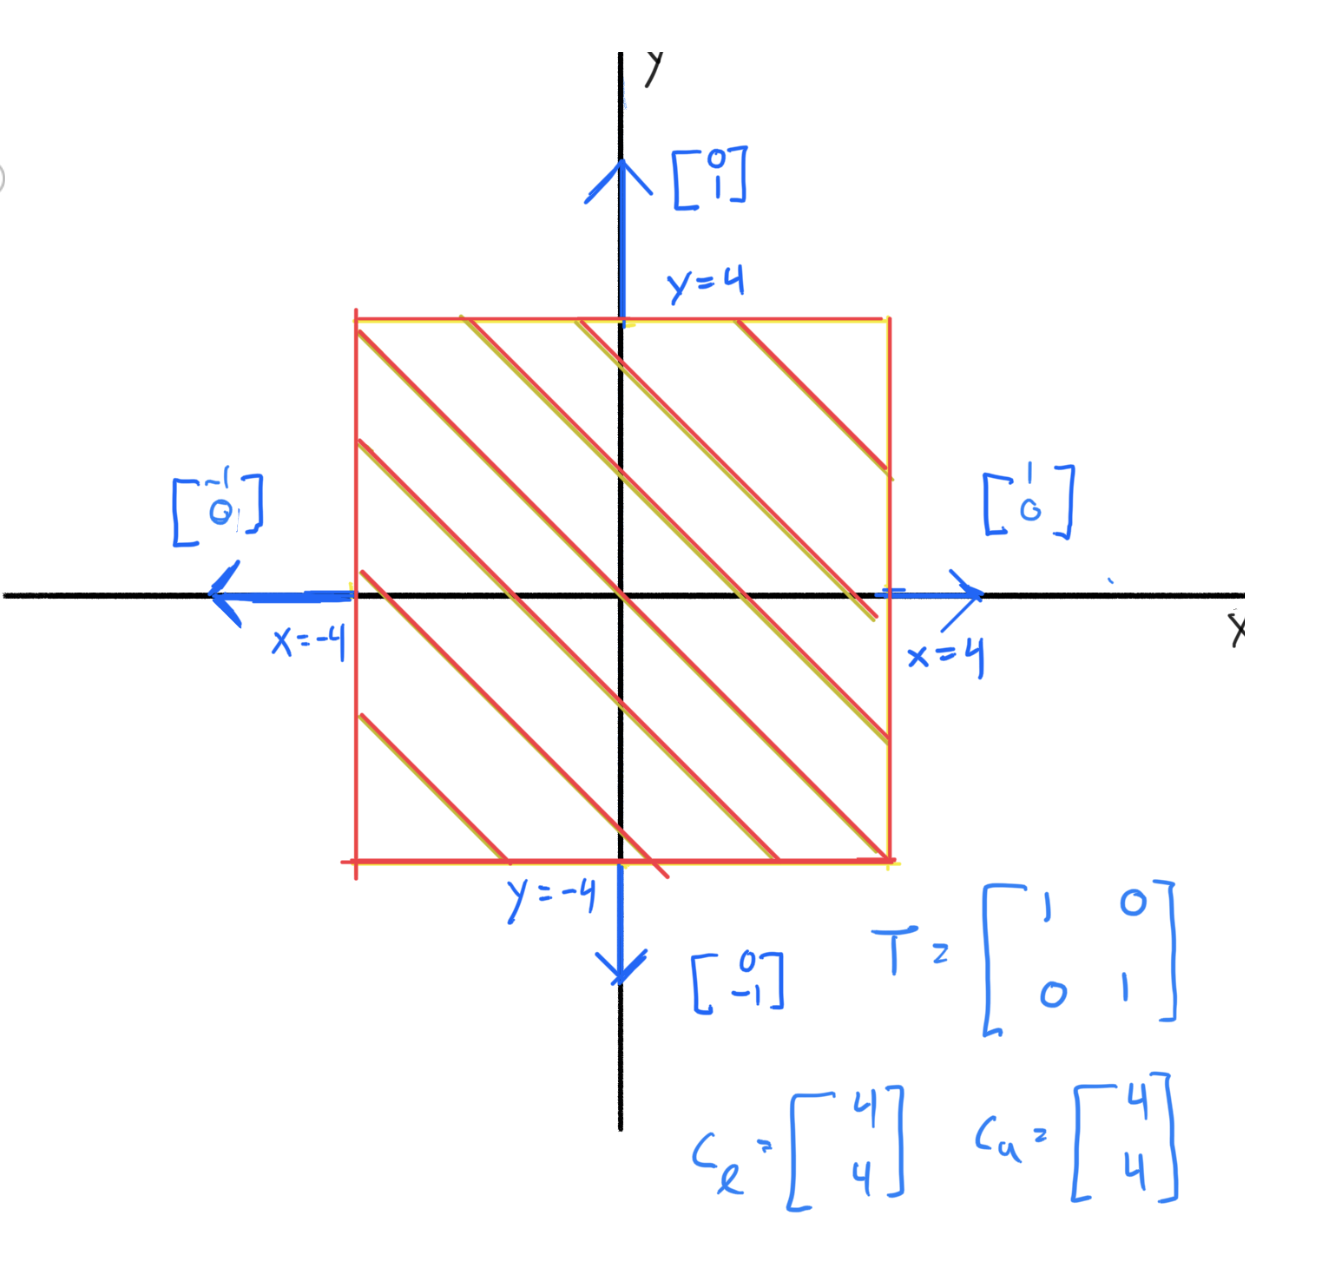
\includegraphics[width=0.6\textwidth]{initptopemat}
    \caption{Example Initial Parallelotope with template matrix and offset vectors.}
  \end{figure}
\end{frame}

\begin{frame}
  \frametitle{\textbf{Background:} Parallelotope Intuition}
  \begin{figure}
    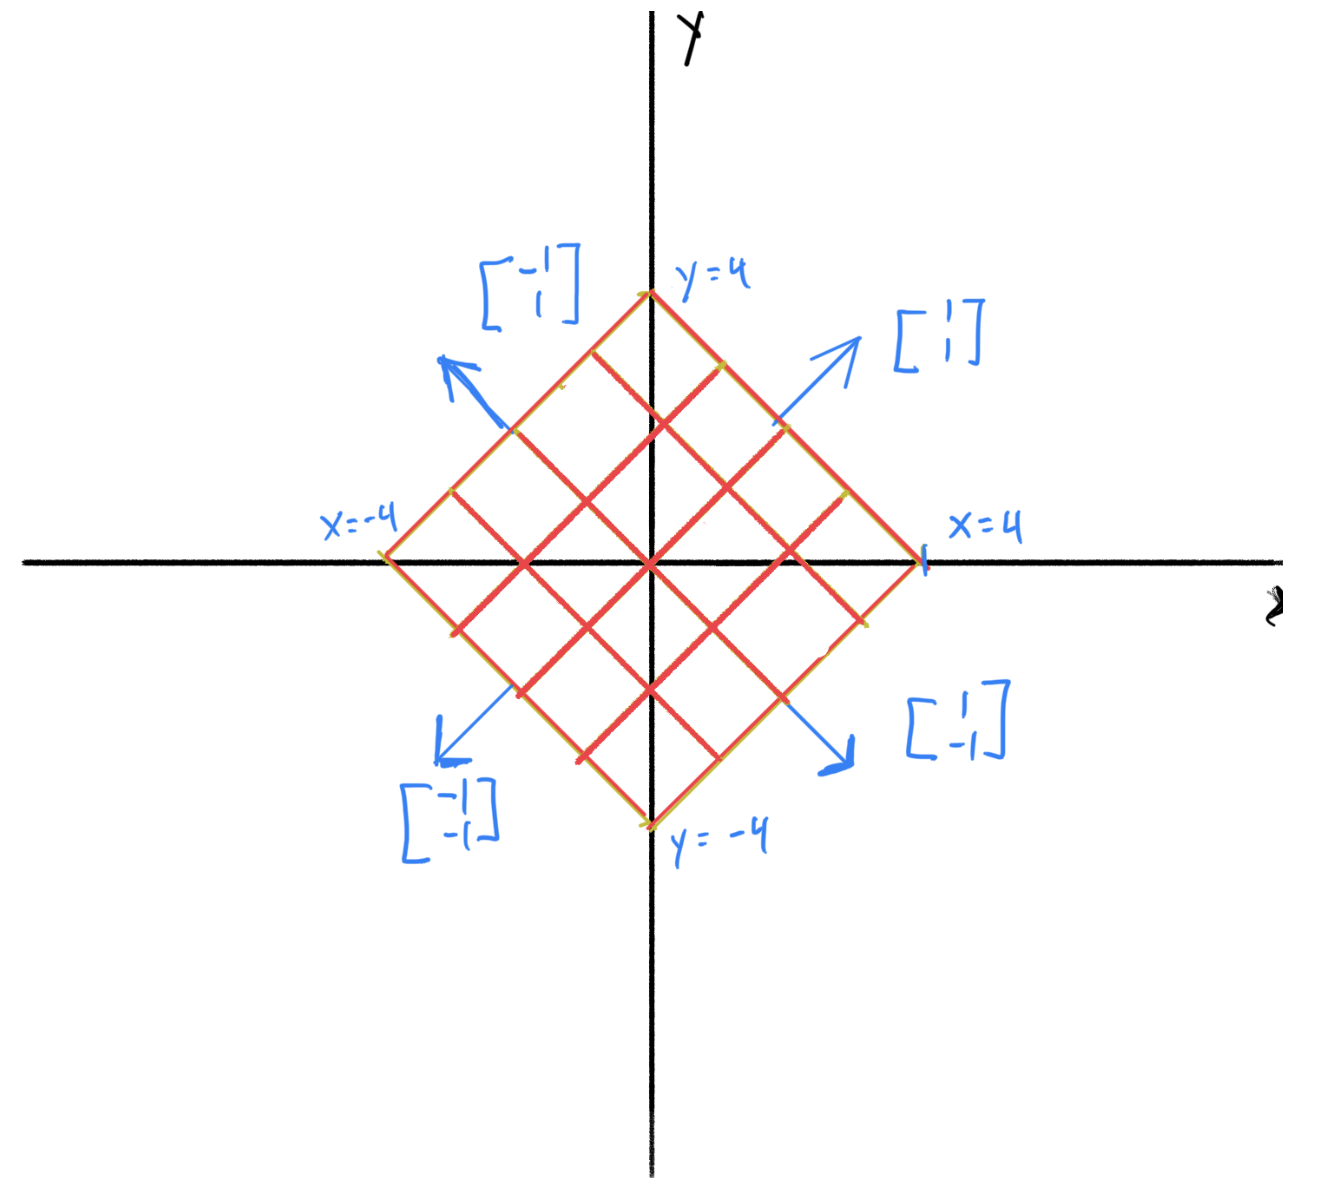
\includegraphics[width=0.7\textwidth]{diagptope}
    \caption{Example Initial Parallelotope rotated 45 degrees clockwise}
  \end{figure}
\end{frame}

\begin{frame}
  \frametitle{\textbf{Background:} Parallelotope Matrices}
  \begin{figure}
    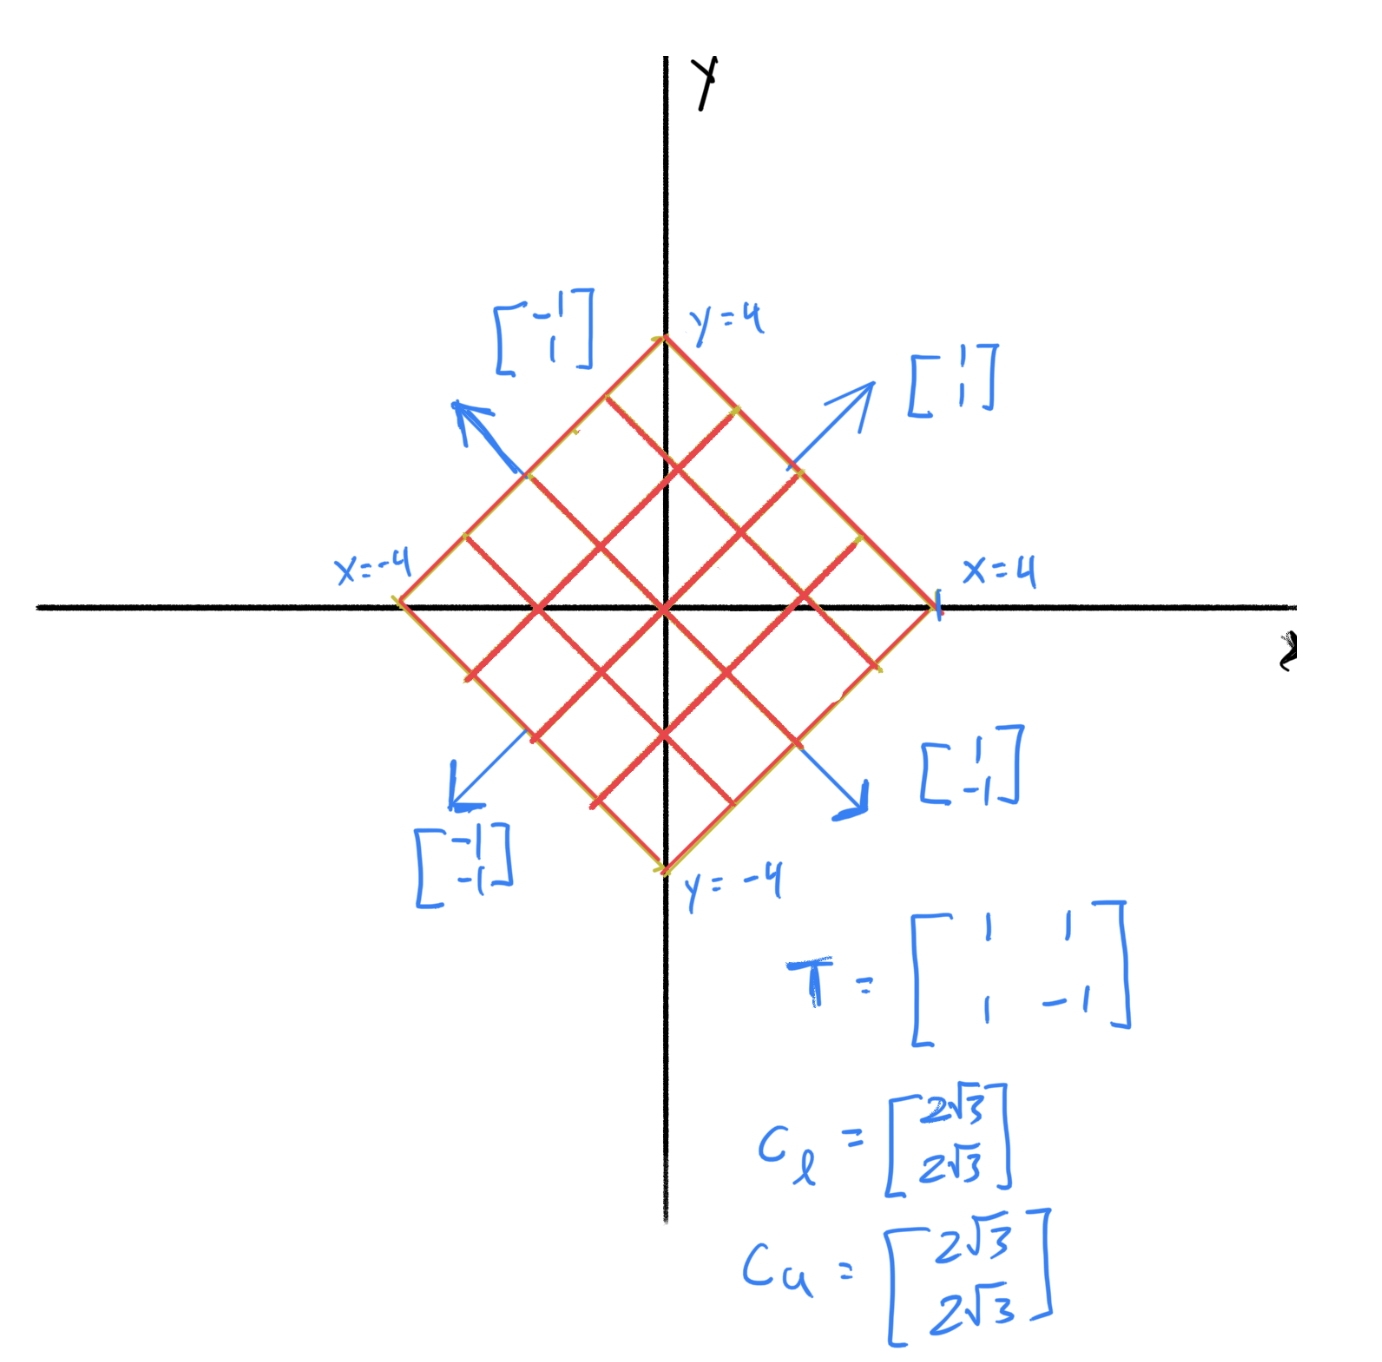
\includegraphics[width=0.6\textwidth]{diagptopemat}
    \caption{Example Rotated Parallelotope with template matrix and offset vectors.}
  \end{figure}
\end{frame}

\begin{frame}
  \frametitle{\textbf{Background:} Parallelotopes}
  \begin{definition}
    A \emph{parallelotope} in $\mathbb{R}^n$ is represented as a tuple $\langle \mathcal{T}, c_{l}, c_{u} \rangle$ where $\mathcal{T} \in \mathbb{R}^{n \times n}$ are called \emph{template directions} and $c_{l}, c_{u} \in \mathbb{R}^{n}$ such that $\forall_{1 \leq i \leq n} ~  c_{l}[i] \leq c_{u}[i]$ are called \emph{bounds}. The half-space representation defines the set of states
    %
    $$
    P = \{\: x \in \mathbb{R}^n \: | \: c_{l}[i] \leq \mathcal{T}_{i}x \leq c_{u}[i], \; 1 \leq i \leq n \}.
    $$
   \end{definition}

   \begin{itemize}
     \item The rows $\mathcal{T}_i$ are called \emph{template directions} in the parallelotope.
     \item Parallelotopes can be thought of cases of template polyhedra where each template direction $\mathcal{T}_i$ has its negative $-\mathcal{T}_i $ also included.
   \end{itemize}
\end{frame}



\begin{frame}
\frametitle{\textbf{Background:} Parallelotope Bundles}
\begin{definition}
  A \emph{parallelotope bundle} $Q$ is a set of parallelotopes $\{P_1, \ldots, P_m\}$. The set of states represented by a parallelotope bundle is given as the intersection
\[ Q = \bigcap_{i=1}^m P_i \]
\end{definition}

\begin{itemize}
  \item We can think of the bundle's template matrix $\mathcal{T}^Q$ as the conjunction of all the template directions $\mathcal{T}_j^{P_i}$ for the $P_i = \langle \mathcal{T}^{P_i}, c_{l}^{P_i}, c_{u}^{P_i} \rangle$
      \item \textbf{Takeaway:} Any convex initial set can be expressed as a parallelotope bundle.
\end{itemize}
\end{frame}

\begin{frame}
  \frametitle{\textbf{Background:} Convex sets can be expressed as Parallelotope Bundles}

  \begin{figure}
    \centering
    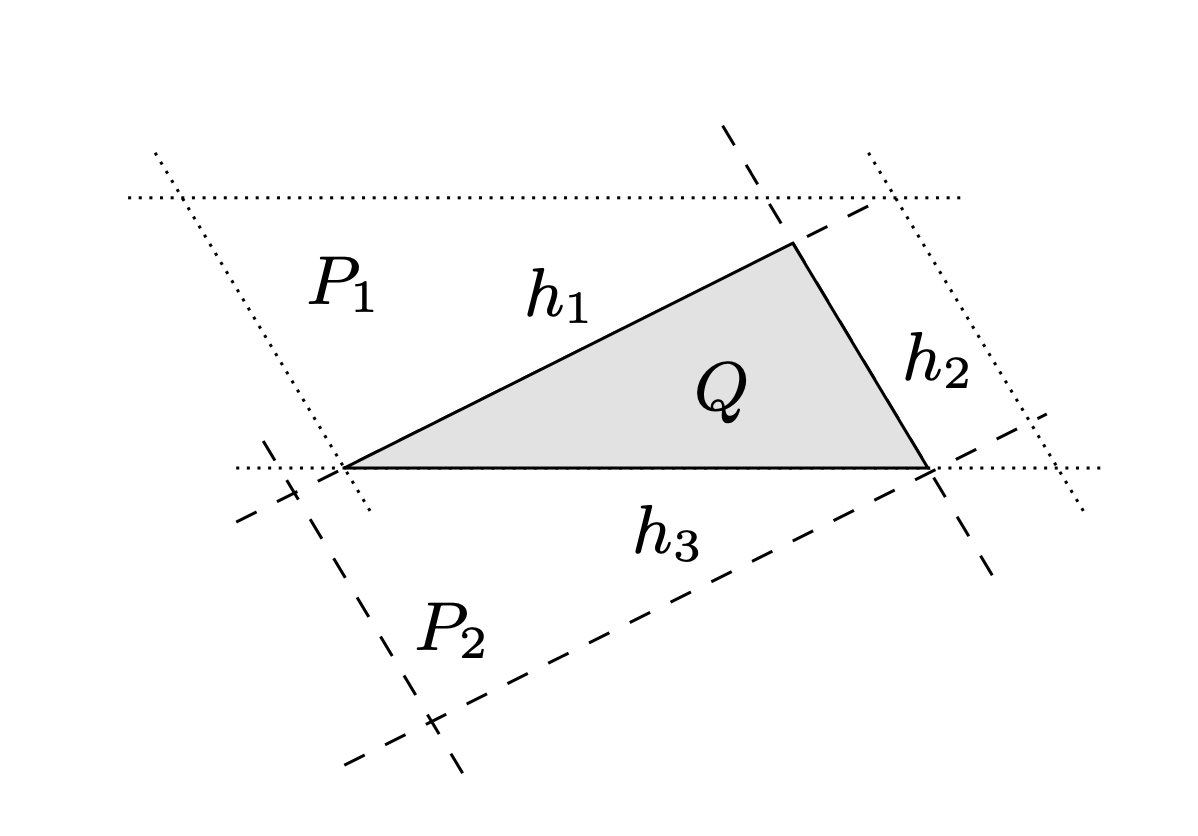
\includegraphics[width=0.65\textwidth]{ptopedecomp}
    \caption{Figure 1 from Dreossi et. al: Parallelotope Bundles for Polynomial Reachability (2016)}
  \end{figure}
\end{frame}

\begin{frame}
  \frametitle{\textbf{Background:} Non-linear Optimization}
  \begin{enumerate}
    \item Consider a parallelotopes $P$ in the bundle $Q$ and a non-linear function $f: \mathbb{R}^n \rightarrow \mathbb{R}^n$. We want to be able to bound the image $f(P)$ using the template directions defining the parallelotopes in our bundle $Q$.

    \item This amounts to finding new upper and lower bound vectors $c_{u}', c_{l}' \in \mathbb{R}^n$ respectively such that
    \[c_{l}'[i] \leq \mathcal{T}^Q_{i}\cdot f(x) \leq c_{u}'[i], \; x \in P \]
    for $1 \leq i \leq n$
  \end{enumerate}
\end{frame}

\begin{frame}
  \frametitle{\textbf{Background:} Non-linear Optimization}
  \begin{enumerate}
    \item The bounds can be formulated as non-linear optimization problems:
   \begin{align*}
     c_{u}'[i] & = \max_{x \in Q} \mathcal{T}^Q_i\cdot f(x) \\
     c_{l}'[i] & = \min_{x \in Q} \mathcal{T}^Q_i\cdot f(x)
   \end{align*}
     \item The reachable set computation is done by iterating this optimization problem to overapproximate the images of the bundles in each step of the computation.
  \end{enumerate}
\end{frame}

\begin{frame}
  \frametitle{\textbf{Background:} Non-linear Optimization}
  \begin{figure}
    \centering
    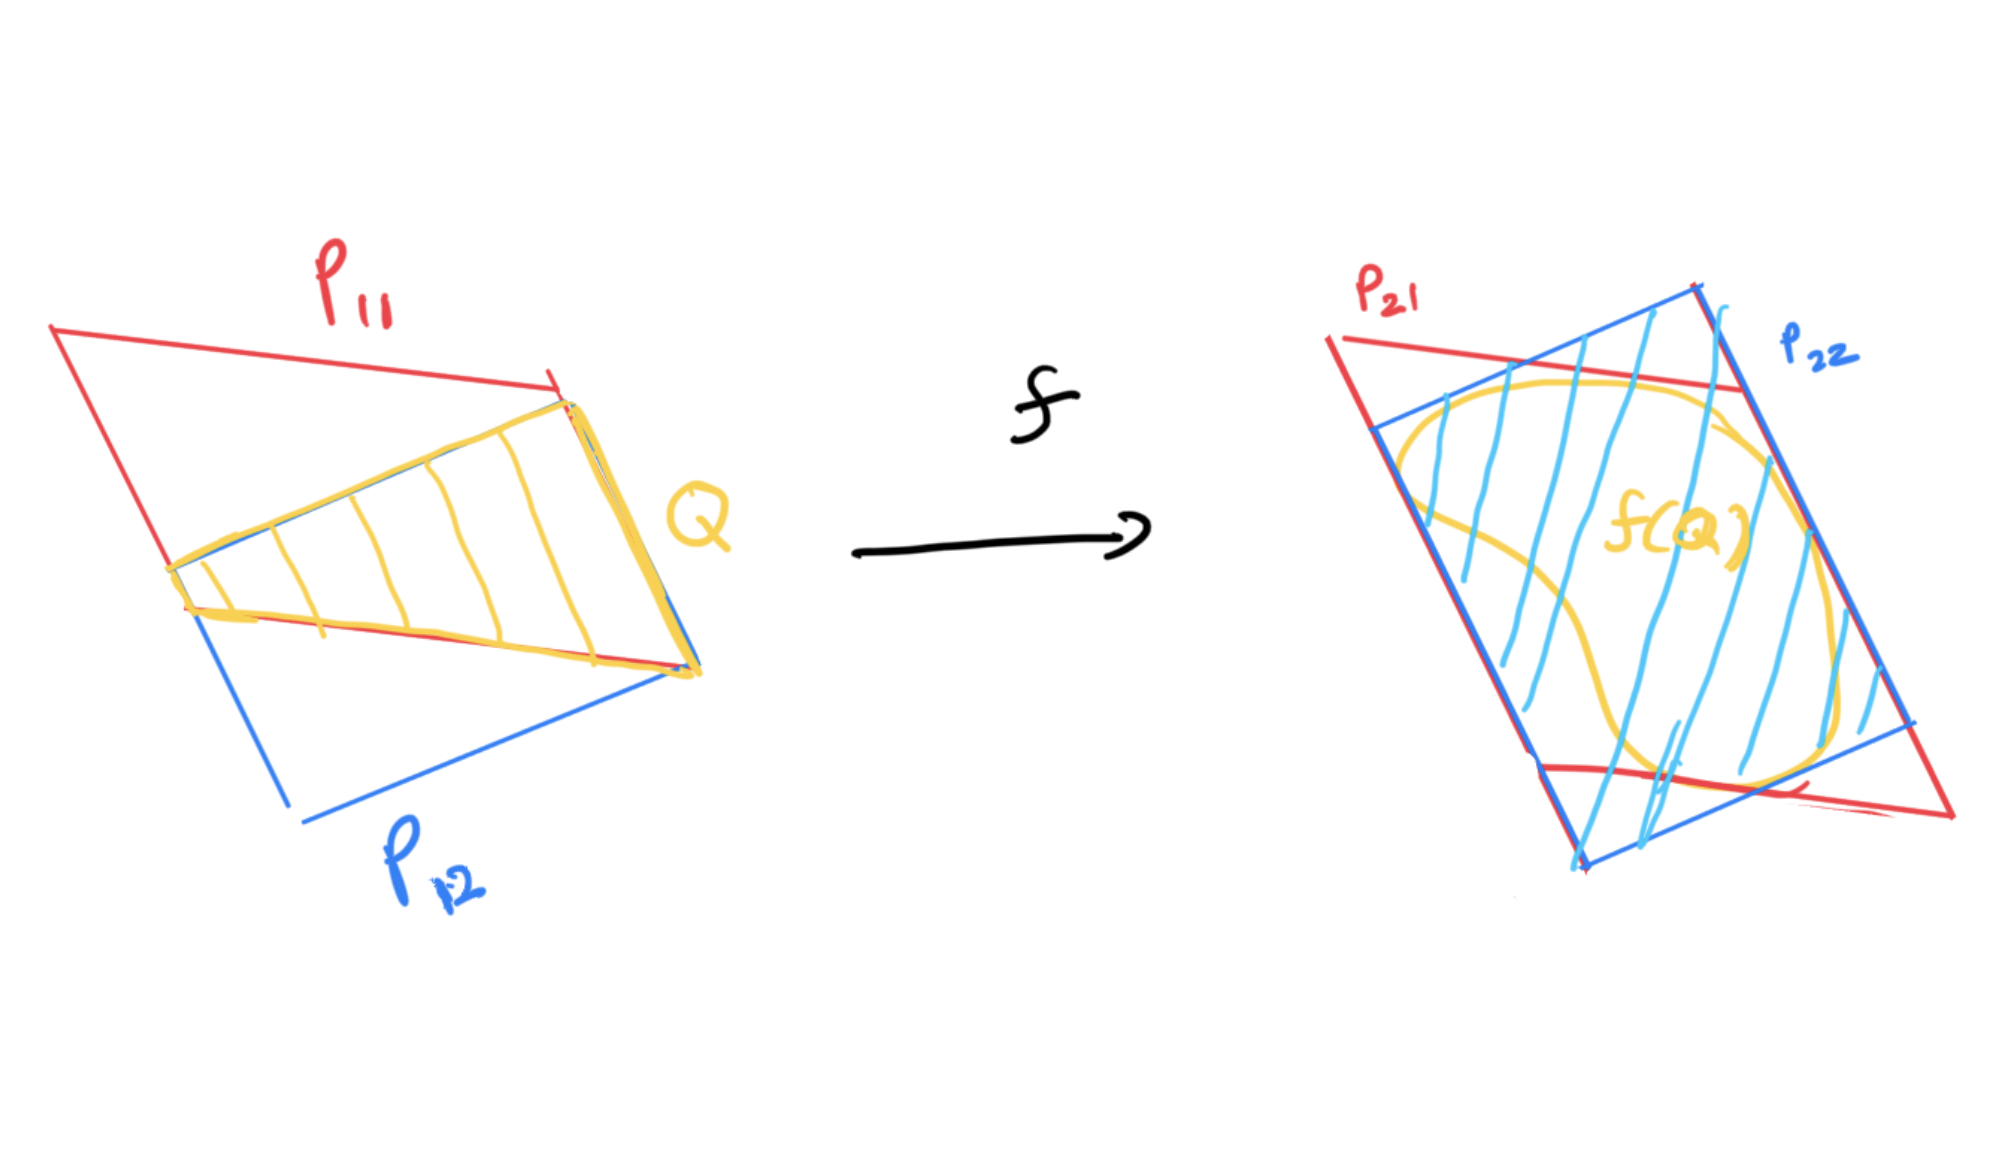
\includegraphics[width=0.65\textwidth]{transformexam}
    \caption{Toy example of the transformation of a bundle containing two parallelotopes}
  \end{figure}
\end{frame}


\begin{frame}
  \frametitle{\textbf{Background:} Algorithm}
  \begin{algorithm}[H] \scriptsize
    \SetKwInput{KwInput}{Input}
    \SetKwInput{KwOutput}{Output}
    \SetKwFunction{AppendPCA}{AppendNewPCATemplates}
    \SetKwFunction{AppendLin}{AppendNewLinAppTemplates}
    \SetKwFunction{TransformBund}{TransformBundle}
    \SetKwFunction{UpdateTemp}{UpdateTemplates}
    \SetKwFunction{GetSupp}{GetSupportPoints}
    \SetKwFunction{PropPoints}{PropagatePointsOneStep}
    \SetKwFunction{PCA}{PCA}
    \SetKwFunction{ApproxLinearTrans}{ApproxLinearTrans}
    \SetKwFunction{SetLifeSpan}{SetLifeSpan}
    \SetKwFunction{AddTemptoBund}{AddTemplateToBundle}
    \SetKwFunction{RemoveTemp}{RemoveTempFromBund}
    \SetKwProg{Fun}{Proc}{:}{}

  \SetAlgoLined
  \DontPrintSemicolon

  \KwInput{Dynamics $f$, Initial Parallelotope bundle $Q_0$, Step Bound $S$, indexes for parallelotopes $I$}
  \KwOutput{Reachable Set Overapproximation $\overline\Theta_k$ for each step $k$} \;

   \For{$k \in [1, 2, \ldots, S]$}{
      $Q_k$ = \TransformBund($f$, $Q_{k-1}$, $\Lambda^{Q_{k-1}}$) \;
     $\overline\Theta_k = Q_k$ \;
   }
   \Return{$\overline\Theta_1 \ldots \overline\Theta_S$} \;
   \;
   %
   \Fun{\TransformBund{$f$, $Q$, $\Lambda$}}{
     $Q' \gets \{\}$; $c_{u} \gets +\infty$; $c_{l} \gets -\infty$\;
     \For{each parallelotope $P$ in $Q$}{
       % $\tup{\T, c_{l}, c_{u}} \gets \mathsf{half-spaceRepresentation}(P)$\;
       \For{each template direction $\Lambda_i$ in the template directions $\Lambda$ }{
         $c_{u}'[i] \gets \mathsf{min}\{ \mathsf{\Lambda_{i} \cdot f}, c_{u}'[i] \}$ \;
         $c_{l}'[i] \gets \mathsf{max}\{\mathsf{-1\times \Lambda_{i} \cdot f}, c_{l}'[i] \}$\;
       }
     }
     Construct parallelotopes $P_{1}', \ldots, P_{k}'$ from $\Lambda, c_{l}', c_{u}'$ and indexes from $I$\;
     $Q' \gets \{P_{1}', \ldots, P_{k}'\}$\;
       % $P' \gets \tup{\T, c_{l}', c_{u}'}$\;
       % $Q' \gets Q' \cup \{P'\}$\;
     \Return{$Q'$} \;
   }
  \end{algorithm}
\end{frame}

\begin{frame}
  \frametitle{\textbf{Background:} Bernstein Expansion}
  \begin{enumerate}
    \item Previous work focused on reachabilty under discrete non-linear \emph{polynomial dynamics} i.e the non-linear function $f: \mathbb{R}^n \rightarrow \mathbb{R}^n$ is polynomial.
    \item Our optimization problems become one of optimizing over polynomial $\mathcal{T}_i\cdot f(x)$ which is generally a costly operation.
    \item The insight comes from leveraging \emph{Bernstein polynomials}. These polynomials yield an efficient manner of bounding the solution to the aforementioned polynomial optimization problems.
    \item An extra linear transformation taking the unit-box domain $[0,1]^n$ to the parallelotope $P$ is required to use Bernstein polynomials.

    %\begin{itemize}
    %  \item Given a polynomial $P$ have the property that their maximum value over the unit box $[0,1]^n$ is upper-bounded by the greatest coefficient
    %\end{enumerate}
  \end{enumerate}
\end{frame}

\begin{frame}
  \frametitle{\textbf{Background:} Drawbacks}
    \begin{columns}
    \column{0.5\textwidth}\scriptsize
    \begin{enumerate}
      \item Hitherto only \emph{static} parallelotopes have been considered. In other words, the template directions specifying the parallelotopes are to be given as user input at the beginning of the reachable set computation.
      \item The template directions chosen are generally the axis-aligned, diagonal directions. However, it's not clear that these directions necessary yield good overapproximations.
      \item Since the template directions are set at the beginning, they cannot adapt to the behavior of the dynamics. This could yield overapproximations which are too conservative for any practical use.
    \end{enumerate}
    \column{0.5\textwidth}
    \begin{figure}
        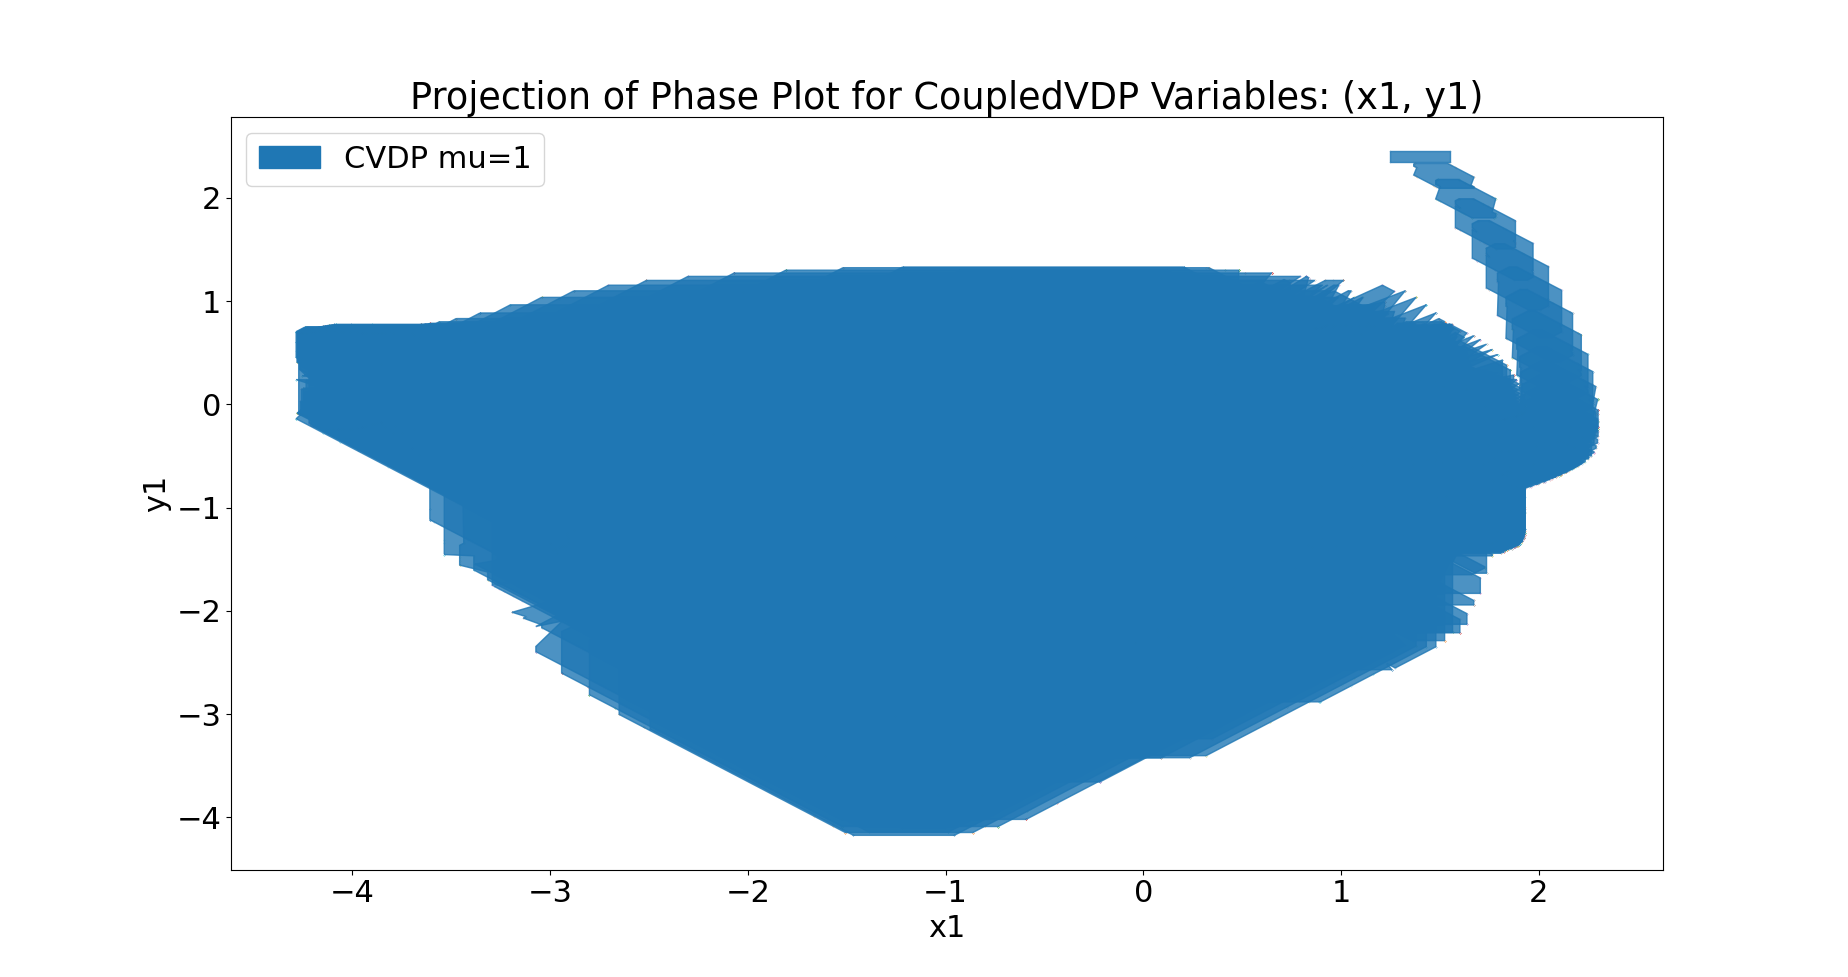
\includegraphics[width=1.13\textwidth]{cvdp20}
        \caption{The effect of choosing inappropriate template directions for the Coupled VanDerPol system.}
      \end{figure}
  \end{columns}
  %Static, diagonal templates are used.
  %Bad for wrapping error as initial sets increase.
\end{frame}

\begin{frame}
  \frametitle{Contributions}
  \begin{enumerate}
    \item We present a method which is both \emph{dynamic} and \emph{automatic}. Our method utilizes the Principal Component Analysis (PCA) and Local Linear Approximations.
    \item  We extend our tool \emph{Kaa} to leverage NASA's \emph{Kodiak} to perform the optimization procedure.
    \item We parallelize our implementation to scale with an increasing number of parallelotopes in our bundles.
  \end{enumerate}
\end{frame}


\begin{frame}
  \frametitle{\textbf{Contributions:} Automatic, Dynamic Algorithm}
  \begin{enumerate}
    \item We choose template directions at each step by two procdure working in tandem
    \item One procedure generates new template directions via Principal Component Analysis (PCA) and the other generates template directions through Local Linear Approximations.
    \item Each procedure adds one parallelotope to the bundle with a set \emph{template lifespan}. This lifespan dictates the future number of steps the parallelotope and its template directions will exist in the bundle.
  \end{enumerate}
\end{frame}


\begin{frame}
    \frametitle{\textbf{Contributions:} PCA Directions}
    \begin{enumerate}
      \item To generate the PCA directions from bundle $Q$, we first calculate the \emph{support points} of all template directions in $\T^Q_i$ over the bundle $Q$.
      \[ p_{i}^u = \max_{x \in Q} T_i^Q \cdot x, \quad  p_{i}^\ell = \min_{x \in Q} T_i^Q \cdot x \]
      \item We then propagate these support points to the next step by the given dynamics $f$. This will gives us set of trajectories.
    \end{enumerate}
\end{frame}

\begin{frame}
    \frametitle{\textbf{Contributions:} PCA Directions}
    \begin{enumerate}
      \item We perform PCA on the endpoints of these trajectories to yield a real-valued $n \times n$ matrix whose rows are the PCA directions. These rows are used as template directions to define a single parallelotope $P'$.
      \item The parallelotope $P'$ with template lifespan $T_{P'}$ is added to the bundle $Q$ to give another bundle $Q' = Q \cup P'$.
    \end{enumerate}
\end{frame}
\begin{frame}
    \frametitle{\textbf{Contributions:} Linear Approx. Directions}
    \begin{enumerate}
      \item Observe that the if the dynamics $f$ were linear i.e $x^+ = Ax$ for some linear transformation $A$, then the image of the parallelotope $c_{l} \leq \T x \leq c_{u}$, will be the set $c_{l} \leq \T \cdot A^{-1} x \leq c_{u}$.
      \item Since the initial parallelotope will be defined by the axis-aligned directions ($\T = I_n$), the image after the first step will be given by
        \[ c_{l} \leq A^{-1} x \leq c_{u}  \]
      Similarly, after the exact image of the initial parallelotope after two steps will problems:
      \[ c_{l} \leq (A^{-1})^2 x \leq c_{u}  \]
    \end{enumerate}
  \end{frame}


\begin{frame}
    \frametitle{\textbf{Contributions:} Linear Approx. Directions}
    \begin{enumerate}
      \item Begin computation with $\T_{lin} = I_n$
      \item To generate the Linear Approximation templates, we once again calculate the support points of all template directions, $\T^Q_i$, over the bundle $Q$.
      \item Propagate the support points using given dynamics $f$ to the next step.   This gives us a set of trajectories $S$.

    \end{enumerate}
\end{frame}

\begin{frame}
    \frametitle{\textbf{Contributions:} Linear Approx. Directions}
    \begin{enumerate}
      \item Calculate the best-fit linear approximation $\mathcal{A}$ using the start and endpoints of the trajectories. Note that $\mathcal{A}$ will be a real-valued $n \times n$ matrix.
      \item Multiply the template directions $\T_{lin}$ by $\mathcal{A}^{-1}$ to yield $\T_{lin} \cdot \mathcal{A}^{-1}$.
      \item Define a parallelotope $P'$ with template lifespan $T_{P'}$ and add it to bundle $Q$ to get $Q' = Q \cup P'$.
      \item $\T_{lin} \gets \T_{lin} \cdot \mathcal{A}^{-1}$
    \end{enumerate}
\end{frame}

\begin{frame}
    \frametitle{\textbf{Contributions:} Template Lifespan}
    \begin{enumerate}
      \item The template lifespan parameter dictates the number of steps after its creation the parallelotope's template directions exist in the bundle.
      \item The intuition is that certain dynamics may be more amenable to directions generated previously in the reachable set computation.
      \item Having a lifespan allows the algorithm to be adaptive while attenuating the computational cost of optimizing over a large number of parallelotopes.
      \item This is a tunable parameter we vary in our experiments.
    \end{enumerate}
\end{frame}

\begin{frame}
    \frametitle{\textbf{Contributions:} Template Lifespan}
    \begin{figure}
      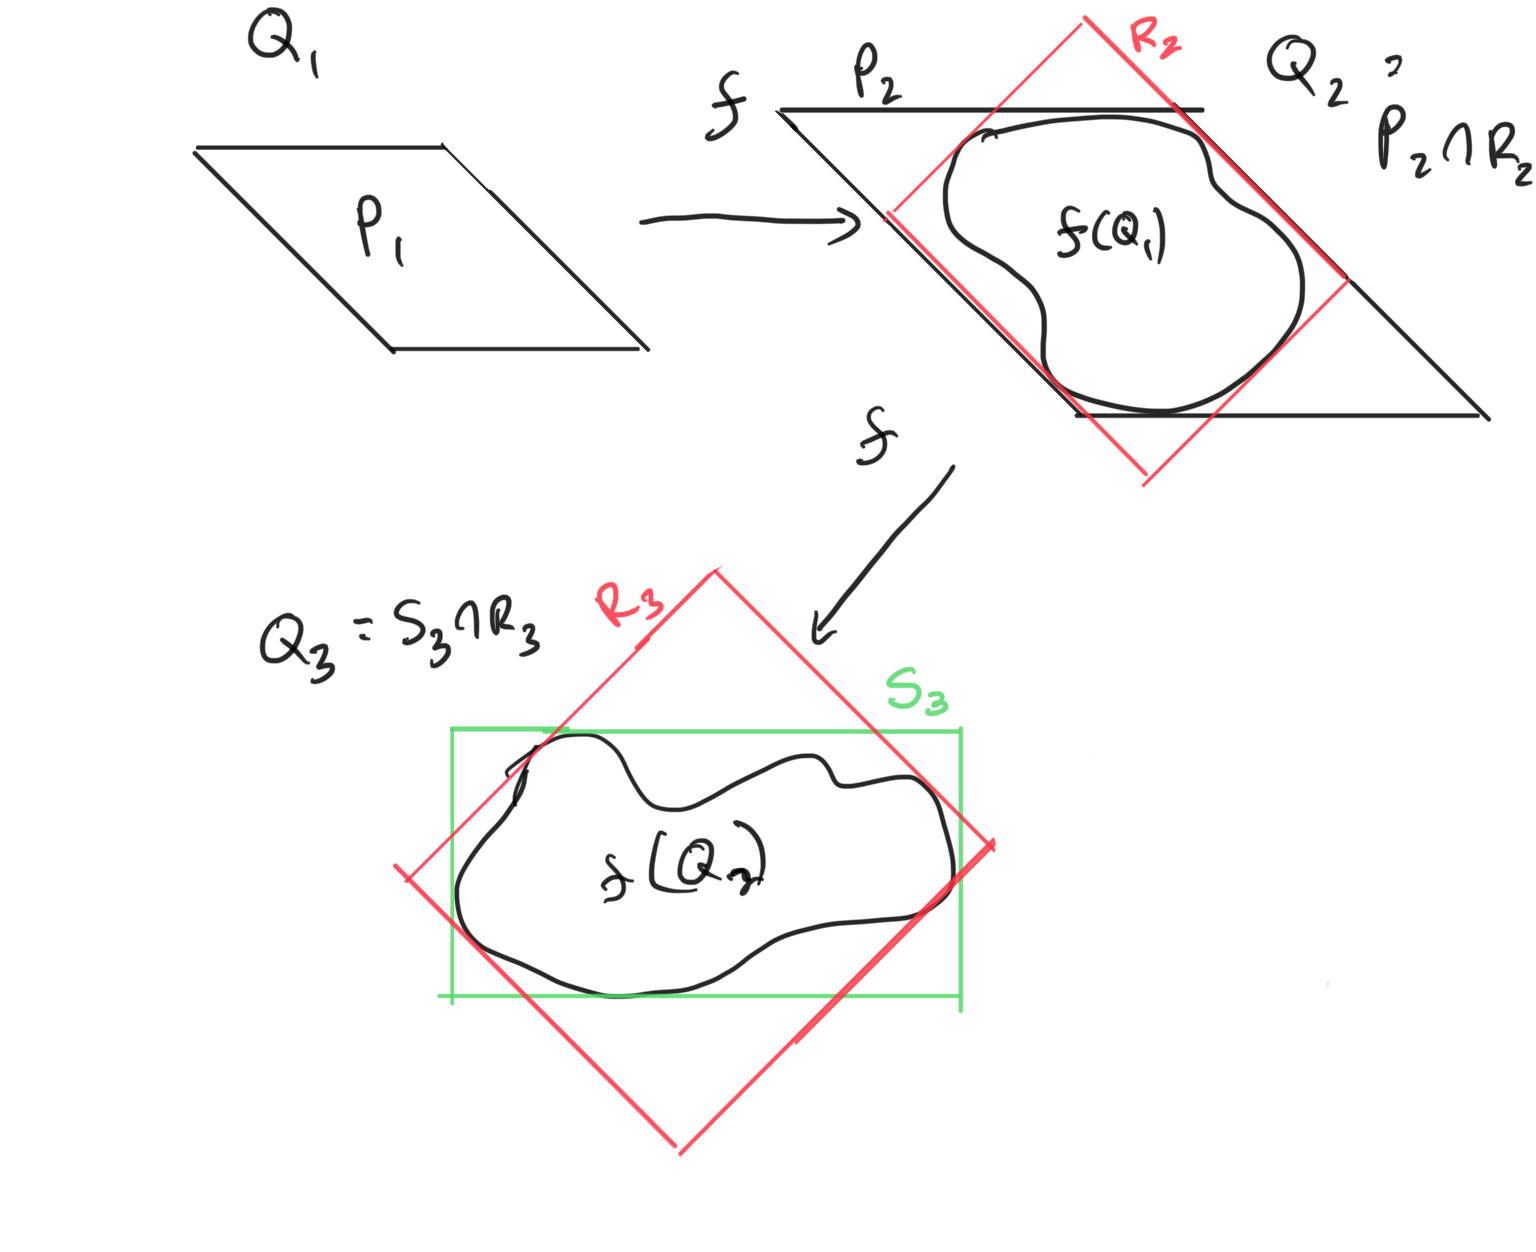
\includegraphics[width=0.7\textwidth]{templifespan}
      \caption{Instance of the template directions of parallelotope $P$ having a template lifespan of two.}
    \end{figure}
\end{frame}


\begin{frame}
    \frametitle{\textbf{Contributions:} Dynamic Algorithm}
    \begin{algorithm}[H] \scriptsize
      \SetKwInput{KwInput}{Input}
      \SetKwInput{KwOutput}{Output}
      \SetKwFunction{CreatePCA}{CreatePCA}
      \SetKwFunction{CreateLin}{CreateLin}
      \SetKwFunction{TransformBund}{TransformBundle}
      \SetKwFunction{UpdateTemp}{UpdateTemplates}
      \SetKwFunction{GetSupp}{GetSupportPoints}
      \SetKwFunction{PropPoints}{PropagatePointsOneStep}
      \SetKwFunction{PCA}{PCA}
      \SetKwFunction{ApproxLinearTrans}{ApproxLinearTrans}
      \SetKwFunction{SetLifeSpan}{SetLifeSpan}
      \SetKwFunction{ExtractDirections}{ExtractDirections}
      \SetKwFunction{AddTemptoBund}{AddTemplateToBundle}
      \SetKwFunction{Maximize}{Maximize}
      \SetKwFunction{hstack}{hstack}
      \SetKwFunction{RemoveTemp}{RemoveTempFromBund}
      \SetKwProg{Fun}{Proc}{:}{}

    \SetAlgoLined
    \DontPrintSemicolon

    \KwInput{Dynamics $f$, Initial Parallelotope $P_0$, Step Bound $S$}
    \KwOutput{Reachable Set Overapproximation $\overline\Theta_k$ at each step $k$}

    $Q_0 = \{P_0 \}$ \;

    % $\T_0 = \{ \{ P_0.\T_1, \ldots P_0.\T_n \} \}$ \;
    $\T = I$ \tcp{Init Template Directions}

     \For{$k \in [1, 2, \ldots, S]$}{
        $P_{supp}$ = \GetSupp($Q_{k-1}$) (support points of $Q_{k-1}$) \;
        $P_{prop}$ = \PropPoints($P_{supp}$, $f$) (image of support points) \;

        $A$ =  \ApproxLinearTrans($P_{supp}$, $P_{prop}$) \; \label{ln:linearapprox}
        $\T = \T \cdot A^{-1}$ \;

        $\T_k^\text{lin} = \{ \T_{1} , \ldots, \T_{n} \} $ \;

        $\T_k^\text{pca} = \{ \PCA(P_{prop}) \} $\; \label{ln:pca}

        $\T_k = \T_k^\text{lin} \cup \T_k^\text{pca}$ \;
        \;
        \tcc{For lifespan $L > 0$, instead call \TransformBund with $\T_k \cup \T_{k-1} \cup \ldots \cup \T_{k-L}$}
        $Q_k$ = \TransformBund($f$, $Q_{k-1}, \T_k$) \;
       $\overline\Theta_k \gets Q_k$ \;
     }
     \Return{$\overline\Theta_1 \ldots \overline\Theta_S$} \;
     %
     \;

    \end{algorithm}
\end{frame}

\begin{frame}
  \frametitle{\textbf{Contributions:} Kaa}
  \begin{enumerate}
    \item Kaa is written in Python and relies on the \emph{numpy} library for matrix computations, \emph{sympy} library for all symbolic subsitution, and \emph{scipy}, \emph{matplotlib} for plotting the reachable sets and computing the volume for lower-dimensional systems.

    \item The optimization procedure for finding the upper and lower bounds of template directions  is performed through the \emph{Kodiak} library. Finally, parallelization of the offset calculation procedures is implemented through the \emph{multiprocessing} module.

    \item Kodiak allows for more general dynamics beyond the polynomial ones considered in a previous tool, \emph{Sapo}
  \end{enumerate}
\end{frame}

\begin{frame}
  \frametitle{\textbf{Results:} Benchmarks}
  \begin{enumerate}
    \item For benchmarking, we select six non-linear models with polynomial dynamics.
    \item Many of these models are also implemented in \emph{Sapo} which explored reachability with {\bf static} parallelotope bundles. In these cases, we directly compare the performance of our dynamic strategies with the Sapo's static parallelotopes defined by \emph{diagonal} directions.
    \item To provide meaningful comparisions, we set the number of dynamic parallelotopes to be equal to the number of static ones excluding the initial box.
  \end{enumerate}
  %Explain benchmarks and choices. Show Table 1
\end{frame}

\begin{frame}
  \frametitle{\textbf{Results:}  Benchmarks}
  %Explain methodology and why we chose this testing procedure with diagonal temps etc.
  \begin{table}[h!]\scriptsize
  %\hspace{-5em}
    \centering
  \begin{tabular}{|p{1.5cm}|c|p{1.7cm}|c|c|p{5cm}|}
  \hline
  Model & Dimension & Parameters & \# steps & $\Delta$  \\
  \hline
  Vanderpol & 2 & \quad \quad \; - & 70 steps & 0.08 \\
  \hline
  Jet Engine& 2 & \quad \quad \; - & 100 steps & 0.2  \\
  \hline
  Neuron & 2 & \quad \quad \; - & 200 steps & 0.2 \\
  \hline
  SIR& 3 & $\beta=0.05$ \newline $\gamma=0.34$ & 150 steps & 0.1 \\
  \hline
  Coupled \newline Vanderpol & 4 & \quad \quad \; - & 40 steps & 0.08 \\
  \hline
  COVID & 7 & $\beta=0.05$ \newline $\gamma=0.0$ \newline $\eta=0.02$ & 200 steps & 0.08 \\
  \hline
  \end{tabular}
  \label{tab:modeldyns}
  \caption{Benchmark models and truncated information}
  \end{table}
\end{frame}

\begin{frame} \small
  \frametitle{\textbf{Results:}  COVID Supermodel}
A modified SIR model accounting for the possibility of asymptomatic patients. Given by the following discretized seven-dimensional dynamics:

\begin{align*}
  \begin{split}
   S_A' & = S_A  -(\beta S_A(A+I))\cdot \Delta \\
   S_I' & = S_I  -(\beta S_I (A + I))\cdot \Delta \\
   A' & = A + (\beta S_I(A+I) - \gamma I)\cdot \Delta \\
   I' & = I + (\beta S_I (A+I) - \gamma I)\cdot  \Delta \\
   R_A' & = R_A + (\gamma A)\cdot \Delta \\
   R_I' & = R_I + (\gamma I)\cdot \Delta \\
   D' & = D + (\eta I)\cdot \Delta
 \end{split}
\end{align*}
where the variables denote the fraction of a population of individuals designated as \emph{Susceptible to Asymptomatic $(S_A)$}, \emph{Susceptible to Symptomatic $(S_I)$}, \emph{Asymptomatic (A)}, \emph{Symptomatic (I)}, \emph{Removed from Asymptomatic $(R_A)$}, \emph{Removed from Symptomatic $(R_I)$}, and \emph{Deceased (D)}.
\end{frame}

\begin{frame}
  \frametitle{\textbf{Results:}  COVID Supermodel}
  \begin{figure}
    \centering
    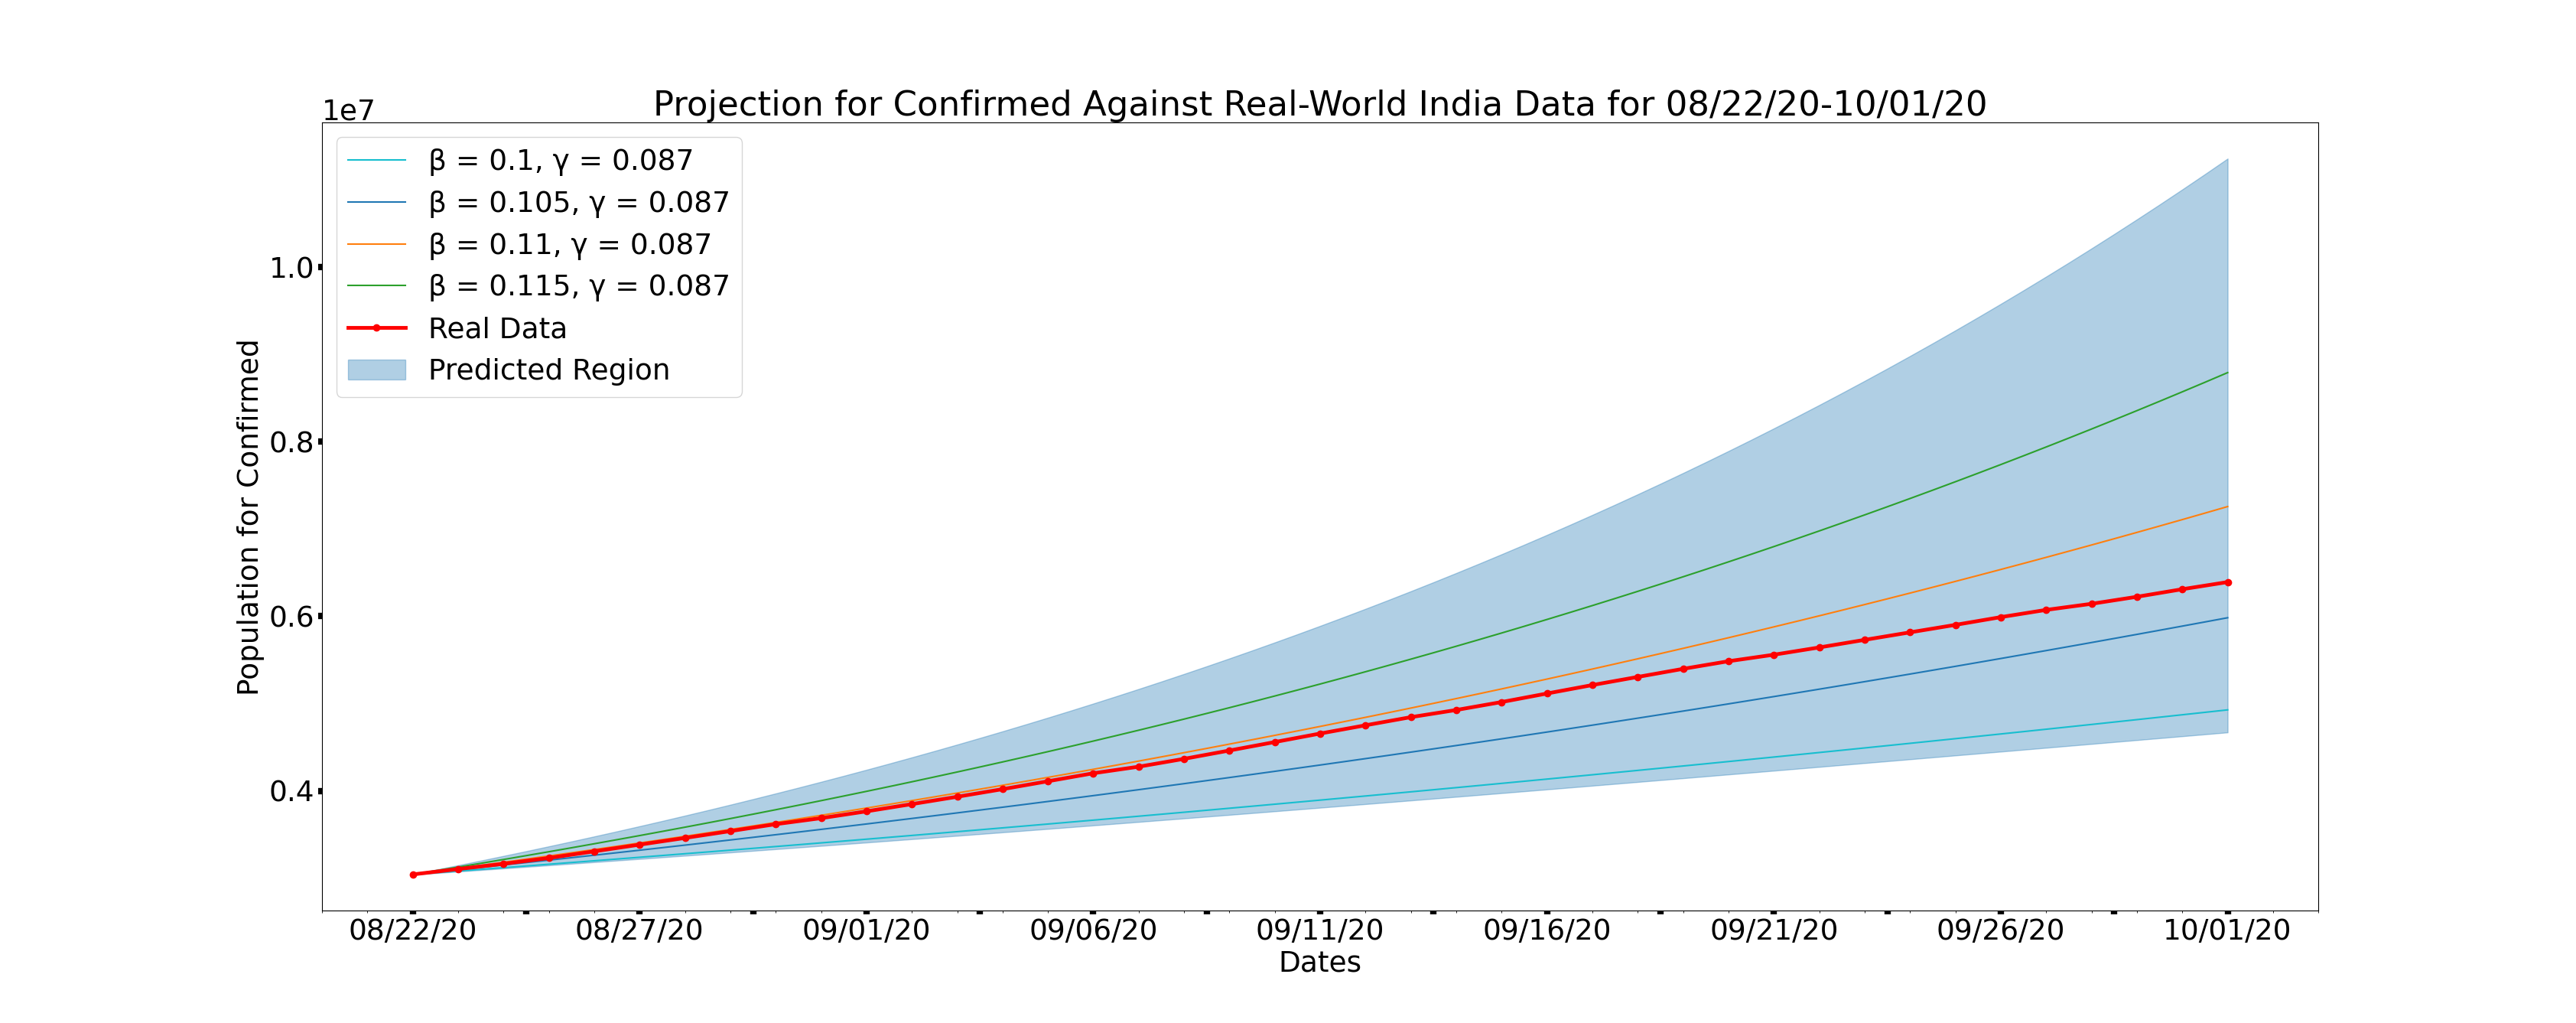
\includegraphics[width=1.1\textwidth]{IndianRecoveredPlot}
    \caption{Plot of COVID Supermodel reachable set against real-world Indian COVID data.}
  \end{figure}
 \end{frame}

\begin{frame}
  \frametitle{\textbf{Results:} Comparision against Static Parallelotopes}
  \begin{columns}
    \column{0.5\textwidth}\footnotesize
    \begin{enumerate}
      \item For models previously defined in Sapo, we set the static parallelotopes to be exactly those found in Sapo.
      \item If a model is not implemented in Sapo, we simply use the static parallelotopes defined in a model of equal dimension.
      \item To address the unavailability of a four dimensional model implemented in Sapo, we sampled random subsets of five static parallelotopes defined with diagonal directions and chose the flowpipe with smallest volume.
    \end{enumerate}
    \column{0.5\textwidth}
    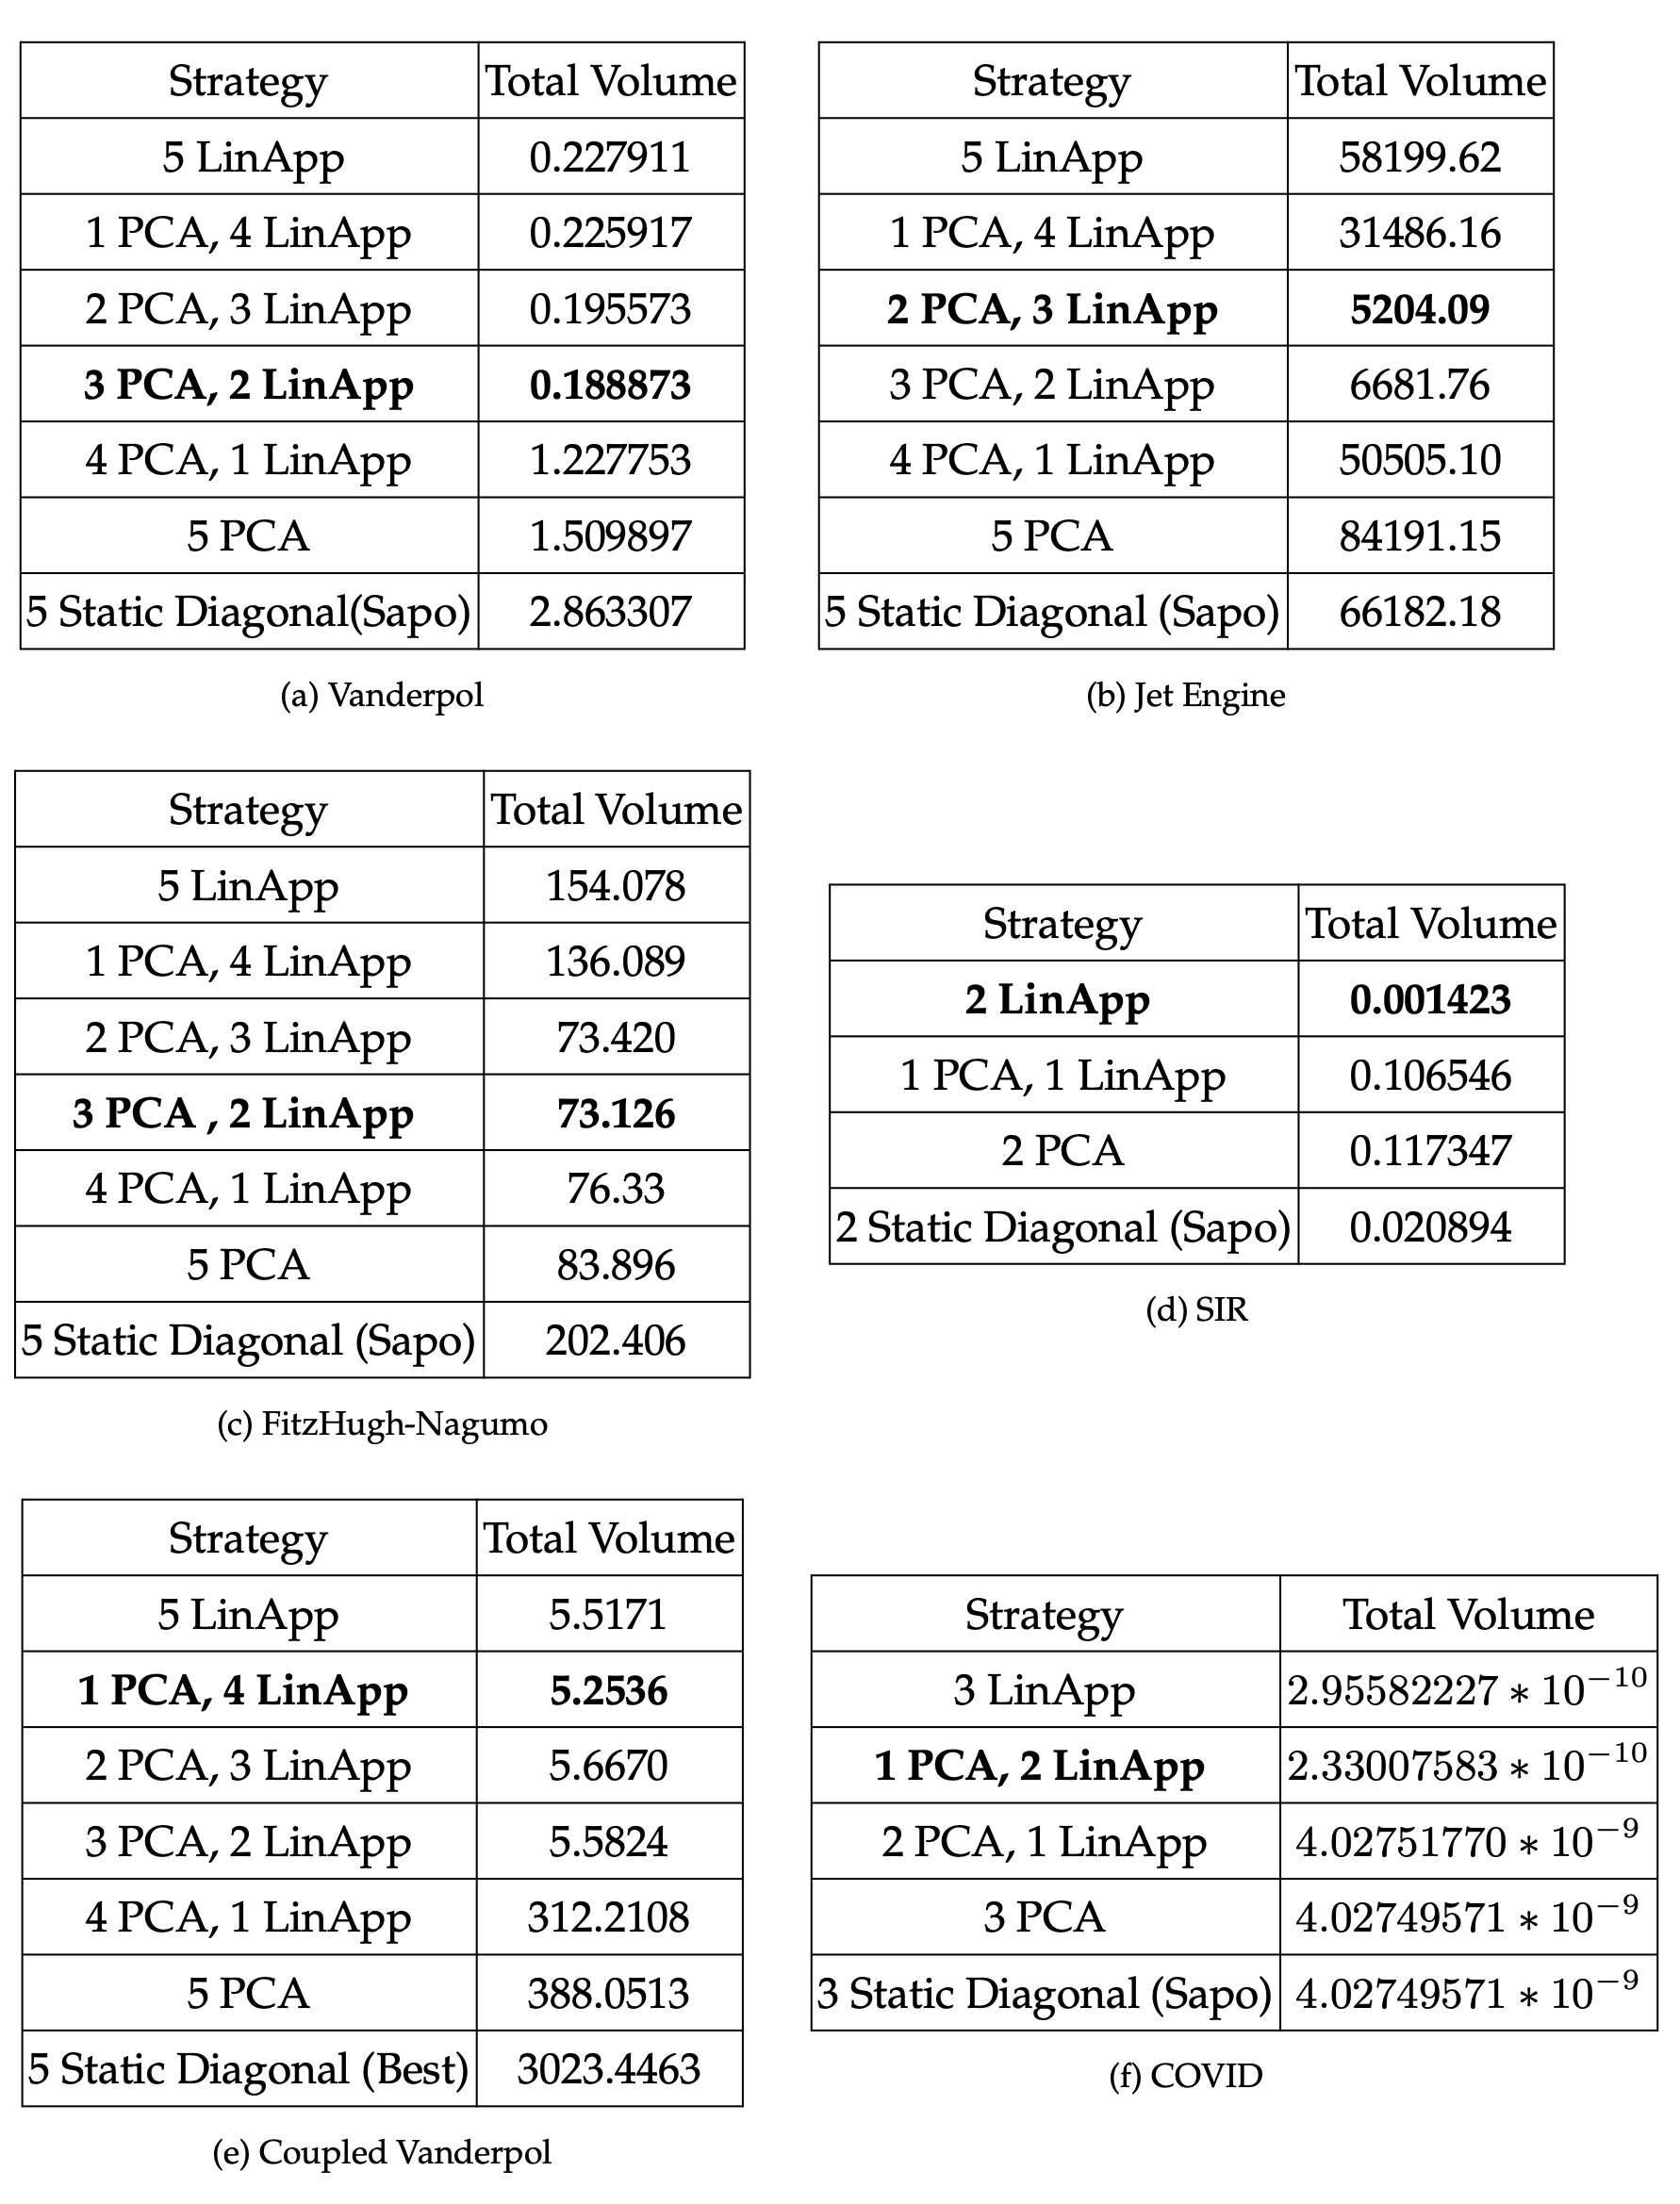
\includegraphics[width=1.05\textwidth]{voltable}
  \end{columns}

\end{frame}


\begin{frame}
  \frametitle{\textbf{Results:}  Performance under Increasing Initial Sets}
  \begin{columns}
      \column{0.5\textwidth}\footnotesize
      \begin{enumerate}
        \item We vary the initial box dimensions to gradually increase the box's volume, then plot the total flowpipe volumes after running the benchmark on the static strategies and best-performing dynamic strategies.
        \item Our dynamic strategies perform better than static ones in controlling the total flowpipe volume as the initial set becomes larger.
        \item The performance of static parallelotopes tends to degrade rapidly as we increase the volume of the initial box
      \end{enumerate}

      \column{0.5\textwidth}
      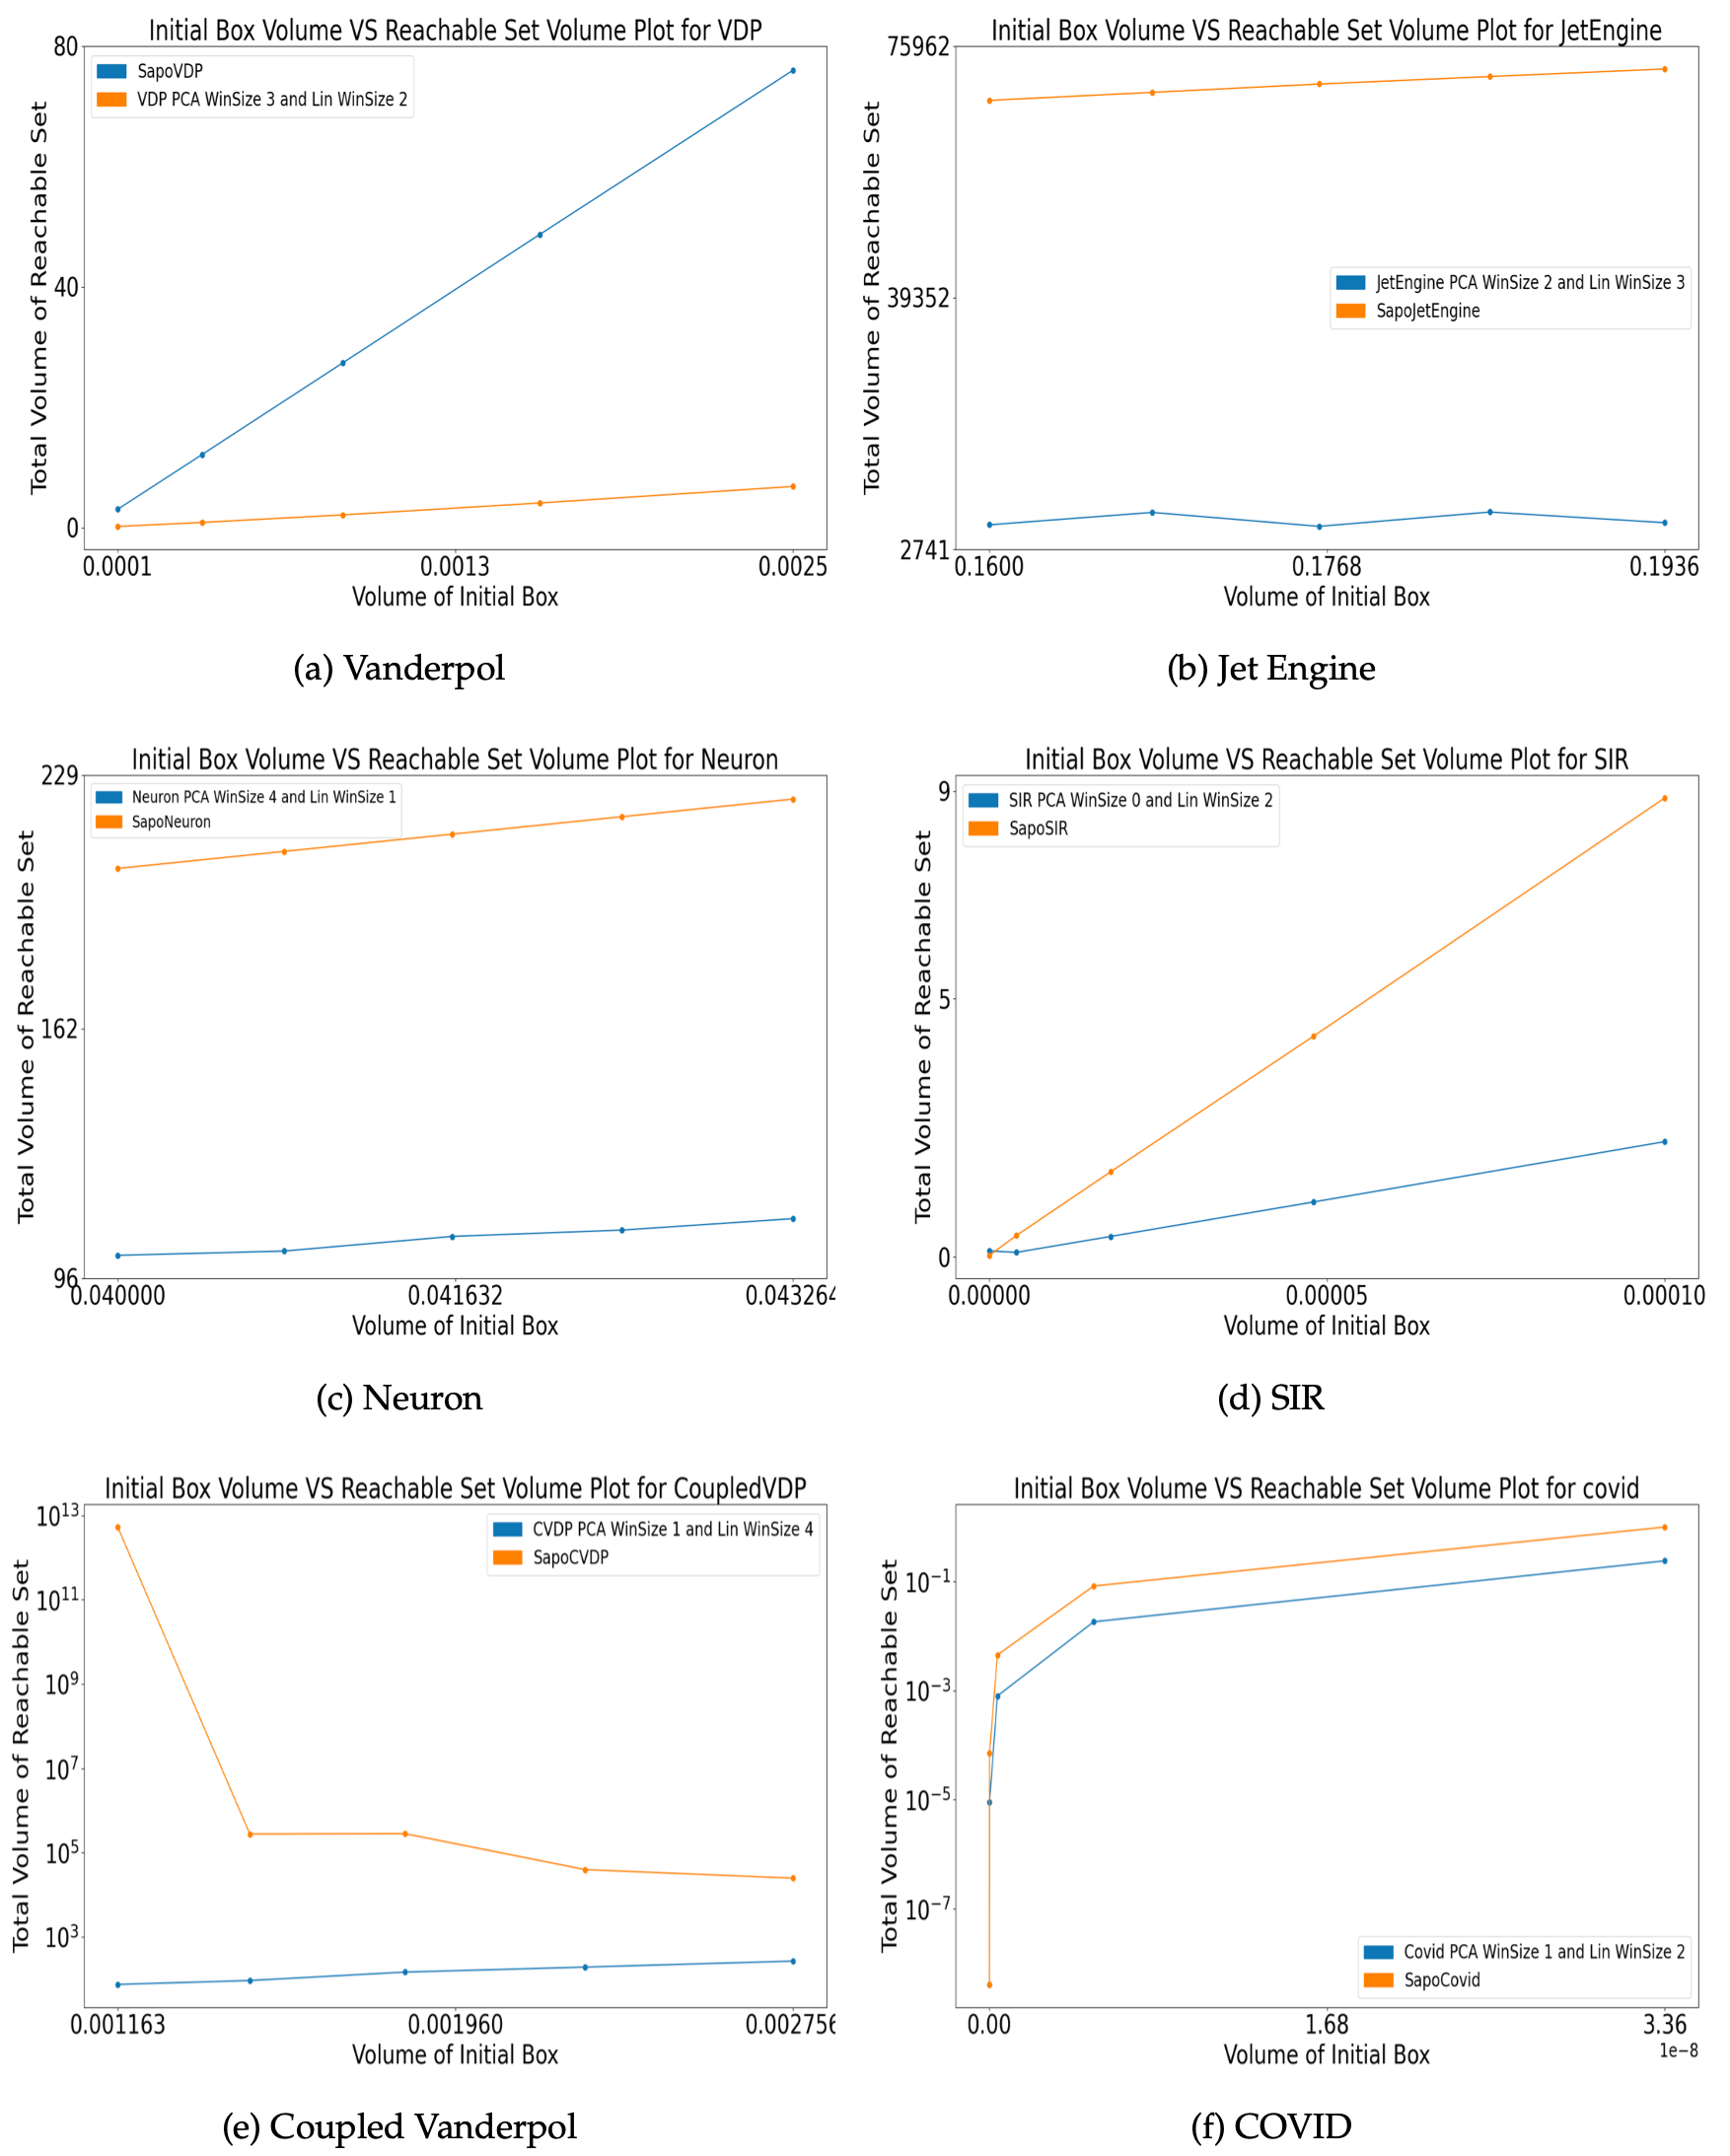
\includegraphics[width=1.1\textwidth]{sapoinitplots}
  \end{columns}
\end{frame}

\begin{frame}
  \frametitle{\textbf{Results:}  Performance against Random Static Bundles}
  \begin{columns}
      \column{0.5\textwidth}\footnotesize
        \begin{enumerate}
          \item We compare our dynamic strategies against static random parallelotope bundles under initial sets with increasing volume.
          \item We sample such parallelotopes in $n$ dimensions by first sampling a set of $n$ directions uniformly on the surface of the unit $(n-1)$-sphere, then defining our parallelotope using these sampled directions
          \item We sample twenty of these parallelotopes for each trial, average the total flowpipe volumes, then plot this against the best-performing dynamic strategy.
        \end{enumerate}

      \column{0.5\textwidth}
      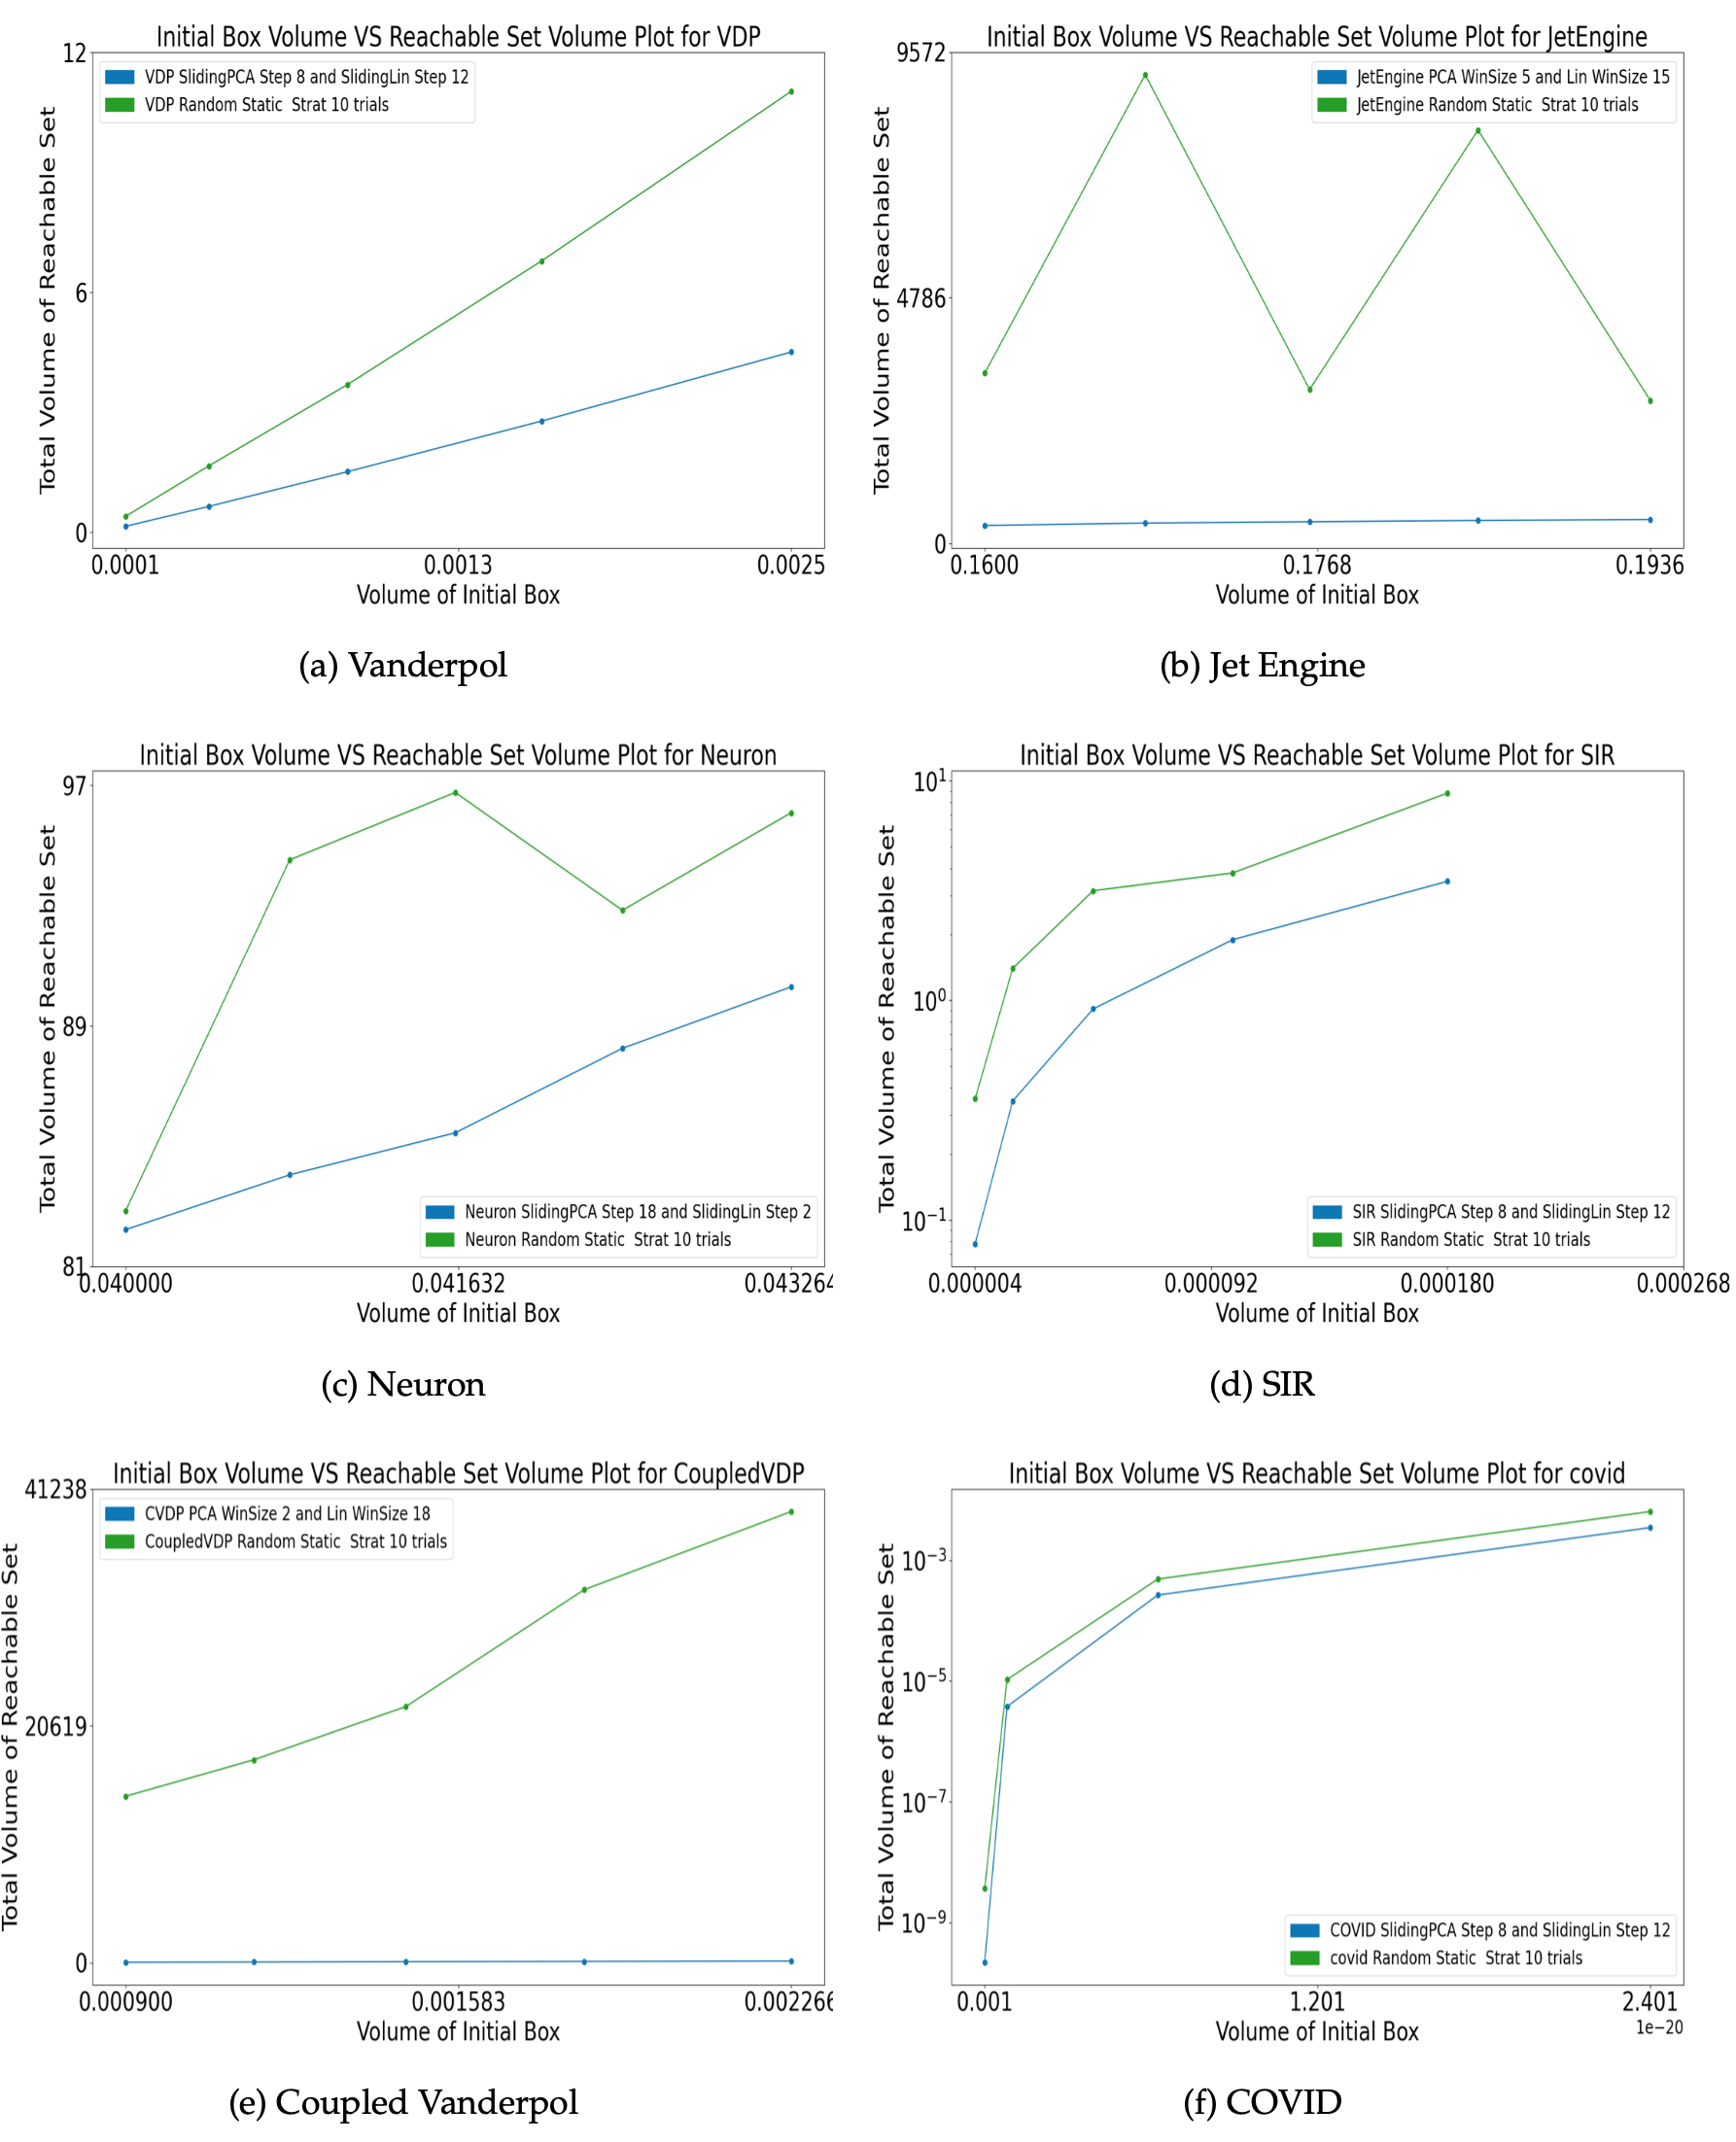
\includegraphics[width=1.1\textwidth]{randomvolplot}
  \end{columns}
\end{frame}


\begin{frame}
  \frametitle{\textbf{Results:}  No Universal Ratio}
  \begin{columns}
      \column{0.5\textwidth}\footnotesize
        \begin{enumerate}
          \item There seems to be no universal optimal ratio between the number of dynamic parallelotopes defined by PCA and Linear Approximation directions which perform well on all benchmarks.
          \item In the Vanderpol model, using parallelotopes defined by Linear Approximation directions is more effective than those defined by PCA directions.
          \item Neuron model shows the opposite trend where using parallelotopes defined by PCA directions is more effective than using those defined by Linear Approximation directions.
        \end{enumerate}
        \column{0.5\textwidth}
        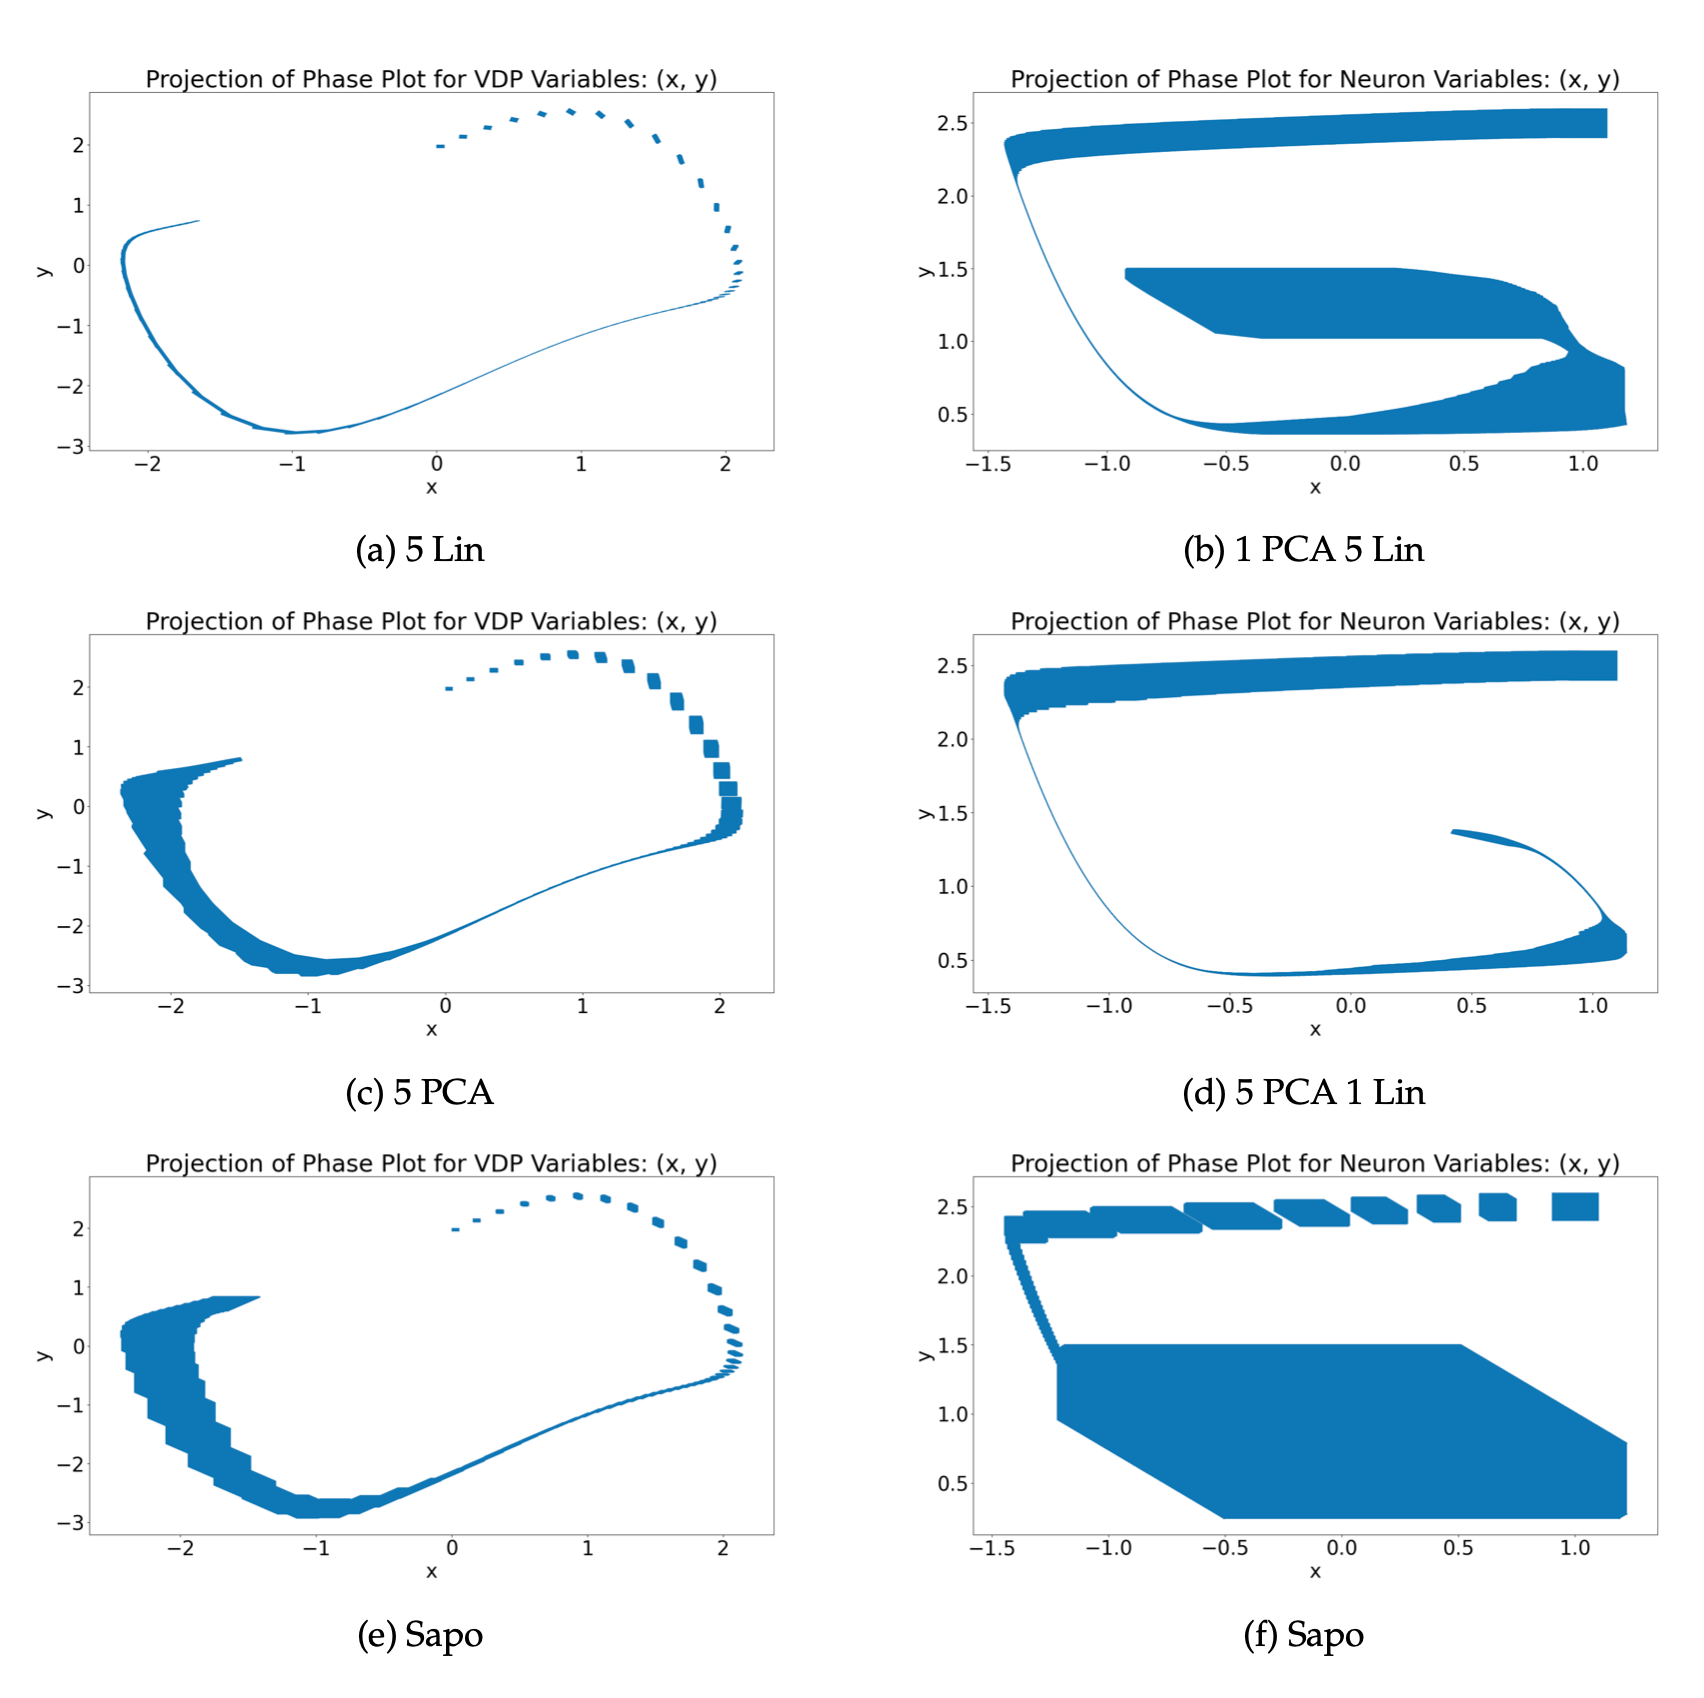
\includegraphics[width=1.15\textwidth]{universalplot}
  \end{columns}
\end{frame}

\begin{frame}
  \frametitle{Future Directions}
  \begin{enumerate}
    \item Are there other adaptive methods we can utilize to generate template directions dynamically?
    \item What about more sophisticated linear approximation methods through Koopman linearization techniques?
    \item The use of massively parallelized reachability techniques through HPC hardware is applicable here. Specifcally, can we leverage GPUs to parallelize the optimization procedure for larger parallelotope bundles?
    \item Why do PCA directions perform better than Linear Approximation directions on certain systems?
  \end{enumerate}
\end{frame}

\begin{frame}
  \frametitle{Concluding Remarks}
  \begin{enumerate}
    \item We investigated two techniques for generating templates dynamically: first using linear approximation of the dynamics, and second using PCA.
    \item We also observed that both these techniques improve the accuracy of the reachable sets for different benchmarks.
    \item We extend Kaa with Kodiak to handle more general dynamics. Systems with more general dynamics are considered in the extended version on arXiv.
  \end{enumerate}
\end{frame}

\begin{frame}
    \frametitle{Relevant Links}
    \begin{itemize}
      \item \textbf{Github Repository for Kaa:} \newline
        https://github.com/Tarheel-Formal-Methods/kaa-dynamic
      \item \textbf{Github Repository for Kodiak:} \newline
        https://github.com/nasa/Kodiak
      \item \textbf{COVID Modeling Blog Post:} \newline
      https://sigbed.org/2021/06/21/sidbed-blog-covid-formal-verification/
    \end{itemize}
\end{frame}

\end{document}
